\documentclass[12pt,a4paper]{report}

% ------------------------------------------------
% PAQUETES
% ------------------------------------------------
\usepackage[utf8]{inputenc}
\usepackage[T1]{fontenc}
\usepackage[spanish]{babel}

% Fuente Times New Roman aproximada
\usepackage{newtxtext,newtxmath}

% Márgenes
\usepackage[
    top=2.5cm,
    bottom=2.5cm,
    left=3cm,
    right=3cm
]{geometry}

% Interlineado 1.5
\usepackage{setspace}
\onehalfspacing

% Espaciado entre párrafos
\usepackage{parskip}
\setlength{\parskip}{6pt}

% Índice
%\usepackage{tocloft}

% Hipervínculos
\usepackage{hyperref}

% Encabezado y pie de página
\usepackage{fancyhdr}
\pagestyle{fancy}

\fancyhf{}
\fancyfoot[C]{\thepage}

% Imágenes
\usepackage{graphicx}

\usepackage{wrapfig}

\usepackage{listings}
\usepackage{xcolor}

\usepackage{booktabs}
\usepackage{tabularx}
\usepackage{makecell}

\lstdefinelanguage{HOC}{
    morekeywords={
        load_file,objref,create,access,forall,
        if,else,for,while,proc,func,begintemplate,
        endtemplate,public,external,strdef,double,
        insert,connect,nseg,L,diam,cm,Ra,v_init,
        run,init,finitialize,fcurrent
    },
    sensitive=true,
    morecomment=[l]{//},
    morecomment=[s]{/*}{*/},
    morestring=[b]"
}

\lstset{
    language=HOC,
    basicstyle=\ttfamily\small,
    keywordstyle=\color{blue},
    commentstyle=\color{green!50!black},
    stringstyle=\color{red},
    numbers=left,
    numberstyle=\tiny,
    frame=single,
    breaklines=true,
    showstringspaces=false,
    tabsize=4
}

% ------------------------------------------------
% FORMATO DE TÍTULOS
% ------------------------------------------------
\usepackage{titlesec}

\titleformat{\chapter}
{\normalfont\Huge\bfseries}
{\thechapter.}{1em}{}

\titleformat{\section}
{\normalfont\Large\bfseries}
{\thesection}{1em}{}

\titleformat{\subsection}
{\normalfont\large\bfseries}
{\thesubsection}{1em}{}

% ------------------------------------------------
% DATOS DEL DOCUMENTO
% ------------------------------------------------
\title{
    \vspace{4cm}
    \textbf{Regulación de las propiedades intrínsecas neuronales por gliotransmisores}\\
    \vspace{1cm}
}

\author{María Calvo Fernández}
\date{\today}

% ------------------------------------------------
% DOCUMENTO
% ------------------------------------------------
\begin{document}

% ------------------------------------------------
% PORTADA
% ------------------------------------------------
\begin{titlepage}
    \centering

    \vspace*{3cm}

    {\Huge \textbf{Regulación de las propiedades intrínsecas neuronales por gliotransmisores} \par}

    \vspace{2cm}

    {\Large María Calvo Fernández \par}

    \vfill

    {\large Centro asociado: CSIC - Centro de Neurociencias Cajal \par}

    {\large Profesor de la Sede Central: Nuria del Olmo Izquierdo \par}

    \vspace{0.5cm}

    {\large Universidad Nacional de Educación a Distancia (UNED) \par}

    {\large \today \par}

    % -------------------------
    % PIE DE PÁGINA EN PORTADA
    % -------------------------
    \vspace{2cm}

    \begin{flushleft}
    \small
    mcalvo584@alumno.uned.es \\
    695 66 24 20
    \end{flushleft}

\end{titlepage}

% ------------------------------------------------
% ÍNDICE
% ------------------------------------------------
\tableofcontents
\newpage

% ------------------------------------------------
% DESCRIPCIÓN DEL CONTEXTO
% ------------------------------------------------
\chapter{Descripción del contexto}

Las prácticas se realizaron en el Instituto Cajal de Neurociencia del CSIC, dentro del grupo de investigación de neurofisiología y plasticidad sináptica de Eduardo Martín. 

El estudio de estos fenómenos se engloba en el campo de la neurociencia, ligándose con la psicología en el área de neuropsicología, que pretende unificar dos niveles de estudio: por un lado el conocimiento biológico de las bases neuronales del cerebro, y por otro, el estudio de las funciones cognitivas superiores. Busca integrar el componente más fisiológico del funcionamiento cerebral con el comportamental, buscando relaciones entre ambos fenómenos y pretendiendo ofrecer teorías explicativas.

El laboratorio investiga acerca de la transmisión y plasticidad sináptica, y en particular las redes neurona-astrocito que se forman en el hipocampo. La actividad astrocitaria es importante en la modulación de la excitabilidad neuronal, y por tanto en la capacidad de respuesta de la neurona, y se han estudiado previamente distintos mecanismos de acción para este fenómeno. Pendiente ha quedado el desarrollo de un modelo computacional que pueda dar base a las explicaciones propuestas hasta el momento, y que tenga cierto poder predictivo sobre cómo a nivel mecanicista el astrocito influye sobre la excitabilidad.

En este proyecto, el objetivo era educarme al respecto de este funcionamiento cerebral, iniciando la aproximación hacia el campo más neurocientífico que psicológico. En concreto, se buscaba realizar un ejercicio de aprendizaje mediante el desarrollo de un modelo computacional que fuese capaz de simular el comportamiento de redes neuronales-astrocitarias del hipocampo, basándose en literatura previa y modelos previamente publicados como ejemplos. Este trabajo se enmarcaba en un estudio previo publicado por el grupo de investigación que reflejaba en detalle los mecanismos celulares y moleculares de la acción del astrocito sobre neuronas piramidales CA1. En él, se analizaba la cadena de sucesos que se da desde que el astrocito es estimulado hasta que cambia la excitabilidad de la neurona a través de distintas corrientes iónicas, resultando en cambios en la IAHP (\textit{after-hyperpolarization potential current}) y en particular su componente lento (sIAHP). Se buscaba usar este conocimiento como base para desarrollar el modelo de simulación de este sistema.


% ------------------------------------------------
% ACTIVIDADES DESARROLLADAS
% ------------------------------------------------
\chapter{Actividades desarrolladas}
Las actividades pueden articularse en tres bloques para la exposición, pero las tres fueron desarrolladas de manera solapada en el tiempo.

\section{Lectura de artículos, investigación previa sobre el tema}

Primero se dedicó tiempo a la lectura y aprendizaje de los conocimientos teóricos básicos y necesarios para la realización de las prácticas. Los conceptos principales incluyeron las neuronas y sus propiedades intrínsecas, así como el conocimiento a alto nivel de las técnicas de experimentación en neurociencia. Se profundizó más en el detalle de las neuronas piramidales del hipocampo y cómo estas forman redes neuronales con otros tipos de neurona como las interneuronas y células gliales como los astrocitos. En particular, se leyeron artículos acerca de cómo estos tres tipos de elementos interactúan entre sí para generar actividad integrada en el tiempo, actividad oscilatoria y ondas cerebrales. Dos de las bandas de actividad propias del hipocampo de la rata son la actividad de bandas theta y gamma, ambas con distintas asociaciones funcionales y conductuales, las cuales se han investigado en relación a la actividad de las interneuronas y astrocitos antes mencionados. Se estudió el detalle de los mecanismos involucrados en estos fenómenos, incluyendo los tipos de iones involucrados, canales, corrientes, ligandos, etc. Finalmente, la formación se complementó con estudios previos de modelos computacionales usados para estudiar distintas partes del hipocampo, astrocitos, actividad oscilatoria, etc.

\subsection{Desarrollo de modelos propios}

Dadas las limitaciones de tiempo y conocimiento, se optó por usar modelos previamente publicados que compartiesen elementos con las tareas a desarrollar. 

Se empezó con modelos simples de neuronas hipocampales para familiarizarse con el software NEURON y su lenguaje de programación. Estos modelos permitieron el estudio de cómo definir una neurona simple y sus componentes (por ejemplo, dividida en soma y dendritas), así como la generación de eventos relevantes de simular, como la inyección de corriente – o voltaje – en el soma de la neurona simulada para estudiar su respuesta. Incluían definición de canales iónicos de sodio y potasio principalmente, así como dinámicas intracelulares de la neurona, definidas en cada caso para el estudio en particular y sus objetivos.

Estos modelos fueron difíciles de ampliar para incluir elementos más detallados como canales iónicos especializados, parametrización de distintas corrientes iónicas, etc. por lo que se pasó a usar modelos más complejos en la cantidad de elementos que simulaban. Se encontraron distintos modelos muy detallados y pormenorizados que resultaron ser demasiado complejos para la tarea en curso, pero finalmente tras hacer distintas pruebas, se optó por usar un modelo con un equilibrio entre simplicidad y potencial de ampliación (Manara et al., 2025).


\subsection{Resultados}

El modelo de base de Manara et al., se desarrolló para adaptarlo a las necesidades del proyecto. Por un lado, se alteró el tipo de estimulación que se usaba: por un lado se simuló una estimulación de corriente inyectada condicionada al retorno al reposo de la neurona simulada, y por otra, una estimulación continua en el tiempo – ambas para estudiar desde distintas aproximaciones la respuesta neuronal bajo distintas condiciones. Por otro lado, se añadió un canal necesario para estudiar la IAHP, fenómeno que se quería estudiar. Este canal fue un canal de potasio dependiente de calcio, por lo que se modelaron los parámetros de dinámicas y mecanismos implicados en el funcionamiento del canal, atendiendo a datos fisiológicos y adaptándolos dentro de lo posible al marco programático. Finalmente, se incluyó también un elemento “astrocitario”, en cuanto a que replicaba funcionalmente lo que sería la actividad astrocitaria sobre este tipo de neuronas piramidales, para poder estudiar la respuesta neuronal diferencial según la presencia o no de actividad glial. Esta aproximación fue una simplificación de los mecanismos específicos de acción del astrocito debido a su complejidad, implicando largas cadenas de pasos que escapaban al alcance del proyecto. Se optó por reflejar su influencia sobre la neurona mediante cambios en los niveles intracelulares de calcio, actuando sobre los canales de calcio de membrana. 

Sobre este modelo se realizaron los análisis de distintas condiciones. Se estudió la aparición de bursts de actividad, la aparición de sIAHP una vez añadido el canal correspondiente, así como un análisis de la actividad oscilatoria que podía surgir bajo determinadas condiciones, y cómo esta cambiaba una vez se incluía el componente astrocitario. 


% ------------------------------------------------
% INFORME DE INVESTIGACIÓN
% ------------------------------------------------
\chapter{Informe de investigación}

\textbf{Resumen}: La excitabilidad intrínseca de las neuronas hipocampales depende de múltiples corrientes iónicas que regulan la frecuencia de disparo y la dinámica oscilatoria neuronal. Entre ellas, las corrientes de post-hiperpolarización (IAHP), particularmente la componente lenta (sAHP), desempeñan un papel central en la adaptación neuronal. Asimismo, evidencias recientes sugieren que la actividad astrocitaria podría modular estos procesos mediante mecanismos lentos dependientes de calcio. En este trabajo se desarrolló un modelo computacional multicompartmental de una neurona piramidal CA1 implementado en el entorno NEURON, incorporando mecanismos dependientes de voltaje y un canal lento de potasio activado por calcio destinado a reproducir la dinámica funcional de la sAHP. A partir de este modelo se exploró el efecto de distintas conductancias iónicas sobre la excitabilidad neuronal y se implementó una modulación periódica simplificada de canales de calcio como aproximación funcional a la señalización astrocitaria. Los resultados muestran que pequeñas variaciones en la entrada intracelular de calcio modifican la activación de corrientes sAHP y alteran la frecuencia de disparo y la dinámica temporal de la actividad neuronal. Aunque el modelo presenta limitaciones derivadas de su carácter simplificado y de la ausencia de dinámica de red, proporciona una herramienta útil para el estudio exploratorio de mecanismos celulares implicados en la modulación oscilatoria hipocampal.

\textbf{Abstract}: The intrinsic excitability of hippocampal neurons depends on multiple ionic currents that regulate firing frequency and neuronal oscillatory dynamics. Among these, afterhyperpolarization currents (IAHP), particularly the slow component (sAHP), play a central role in neuronal adaptation. Recent evidence further suggests that astrocytic activity may modulate these processes through slow calcium-dependent mechanisms. In this study, a multicompartmental computational model of a CA1 pyramidal neuron was developed in the NEURON simulation environment, incorporating voltage-dependent mechanisms and a slow calcium-activated potassium current designed to reproduce the functional dynamics of the sAHP. Using this model, we explored the effects of different ionic conductances on neuronal excitability and implemented a simplified periodic modulation of calcium channels as a functional approximation of astrocytic signaling. The results show that small variations in intracellular calcium entry modulate the activation of sAHP currents and alter both firing frequency and the temporal dynamics of neuronal activity. Although the model is limited by its simplified representation and the absence of network dynamics, it provides a useful framework for the exploratory study of cellular mechanisms involved in the modulation of hippocampal oscillatory activity.

\textbf{Palabras clave}: CA1, neurociencia computacional, sAHP, astrocito, actividad oscilatoria

\section{Introducción}
La actividad neuronal surge de cambios en el potencial eléctrico de la membrana celular producidos por el flujo de iones a través de canales iónicos especializados. La interacción entre distintas corrientes iónicas determina propiedades fundamentales como la excitabilidad neuronal, la frecuencia de disparo y la aparición de patrones oscilatorios complejos (Bean, 2007).

Las propiedades intrínsecas de excitabilidad emergen de la combinación específica de canales iónicos presentes en la membrana celular, los cuales determinan cómo responde la neurona ante diferentes niveles de estimulación. Entre los mecanismos más relevantes se encuentran las corrientes de adaptación dependientes de calcio. Durante la actividad repetida, la entrada intracelular de calcio puede activar corrientes de potasio responsables de fenómenos de posthiperpolarización (AHP, \textit{afterhyperpolarization)}, reduciendo temporalmente la excitabilidad neuronal (Sah et al., 2002; Pedarzani et al., 2008). Estas corrientes contribuyen a limitar la frecuencia de disparo y generan períodos de recuperación tras episodios de actividad intensa. 

La interacción dinámica entre excitación, acumulación intracelular de calcio y mecanismos de adaptación puede dar lugar a patrones de actividad conocidos como \textit{bursting}, caracterizados por grupos de potenciales de acción separados por períodos de relativa inactividad. Este tipo de dinámica resulta especialmente relevante en neuronas piramidales CA1 del hipocampo, las cuales presentan propiedades capaces de favorecer actividad rítmica y oscilatoria (Stan Leung et al., 1991). Ciertos estudios sugieren que dichas dinámicas dependen no solo de la conectividad sináptica de la red, sino también de mecanismos intrínsecos relacionados con la regulación del calcio intracelular y las corrientes de posthiperpolarización dependientes de calcio (Chen et al., 2005).

Tradicionalmente, las corrientes AHP se han dividido en tres componentes temporales principales: rápida (fAHP), media (mAHP) y lenta (sAHP). La fase rápida ocurre inmediatamente tras el potencial de acción y participa principalmente en la repolarización de la membrana y en la limitación de la frecuencia instantánea de disparo. La fase media, asociada frecuentemente a canales de potasio activados por calcio de tipo BK o SK, contribuye a mecanismos de adaptación de corta duración y al control de la excitabilidad en escalas temporales intermedias (Sah et al., 2002; Pedarzani et al., 2008). La fase lenta o sAHP presenta especial relevancia debido a su capacidad para modular la excitabilidad neuronal durante períodos prolongados, hasta cientos de milisegundos. Este componente surge principalmente como consecuencia de la acumulación intracelular de calcio durante la actividad repetida, lo que activa corrientes lentas de potasio responsables de una hiperpolarización sostenida (Lancaster et al., 1986; Sah et al., 2002). La sAHP desempeña un papel fundamental en la regulación de la frecuencia de disparo, los intervalos entre \textit{bursts} y la estabilidad de la actividad oscilatoria neuronal (Madison et al., 1984; Golomb et al., 2006). Alteraciones en la regulación de la sAHP pueden modificar significativamente la excitabilidad neuronal y la aparición de patrones oscilatorios (Faber et al., 2003).

Aunque tradicionalmente la actividad cerebral se ha interpretado principalmente desde una perspectiva centrada en las neuronas, en las últimas décadas se ha reconocido el papel activo de las células gliales en la modulación de la actividad neuronal (Araque et al., 1999; Perea et al., 2009). Entre ellas, los astrocitos constituyen uno de los principales tipos celulares gliales y participan en múltiples procesos relacionados con la homeostasis del entorno neuronal (Bellot-Saez et al., 2017). Además de sus funciones de soporte, los astrocitos son capaces de responder a la actividad neuronal mediante incrementos de calcio intracelular y la liberación de distintas moléculas señalizadoras, fenómeno conocido como gliotransmisión (Haydon, 2001; Volterra et al., 2005). A través de distintos mecanismos, la actividad astrocitaria puede alterar la excitabilidad neuronal y modificar la dinámica temporal de las redes neuronales (Perea et al., 2007; Semyanov et al., 2020). Algunos estudios sugieren que la señalización glial puede influir sobre procesos oscilatorios y sobre la sincronización de poblaciones neuronales, especialmente mediante mecanismos lentos de modulación de la excitabilidad (Poskanzer et al., 2016). En neuronas hipocampales, estas interacciones podrían afectar indirectamente a la regulación del calcio intracelular y a corrientes dependientes de calcio implicadas en la generación de la sAHP y en el control de los intervalos entre \textit{bursts} (Tzingounis et al., 2008; Semyanov et al., 2020).

En este contexto, resulta relevante estudiar cómo mecanismos lentos de modulación glial pueden alterar las propiedades intrínsecas responsables de la generación de \textit{bursting} y de la actividad oscilatoria neuronal. Debido a la complejidad de las interacciones entre corrientes iónicas, mecanismos dependientes de calcio y modulación glial, los modelos computacionales son una herramienta útil para estudiar de forma controlada cómo distintos parámetros celulares influyen sobre la excitabilidad neuronal y la dinámica oscilatoria.
El objetivo de este proyecto es desarrollar un modelo computacional que permita el análisis de la relación entre la modulación glial, el \textit{bursting} y la actividad oscilatoria, a través de mecanismos de calcio y propiedades intrínsecas de la neurona como la sAHP.

\section{Método}
\subsection{Diseño}
El trabajo consiste en una simulación computacional \textit{in silico} de carácter exploratorio, complementada con una fase final de análisis experimental mediante simulaciones sistemáticas. En la fase exploratoria, se modificaron distintos parámetros del modelo (variables independientes), observándose sus efectos sobre diversas medidas de excitabilidad y dinámica oscilatoria (variables dependientes), con el objetivo de identificar patrones y relaciones sin partir de hipótesis previamente establecidas.
Posteriormente, se realizó una sección de carácter experimental unifactorial centrada en analizar el efecto de la actividad glial (VI) sobre la frecuencia de oscilación neuronal (VD), manteniendo controladas el resto de variables del modelo.

\subsection{Procedimiento}
Primero, se realizó una fase exploratoria orientada a caracterizar la dinámica básica del modelo y ajustar parámetros relacionados con la excitabilidad neuronal, las corrientes de hiperpolarización y posthiperpolarización (IAHP), y la acumulación intracelular de calcio. Posteriormente se implementó un mecanismo de modulación glial lenta mediante una señal oscilatoria aplicada sobre la conductancia cálcica neuronal. Esta señal representaba de forma funcional la influencia astrocitaria sobre la excitabilidad neuronal. Finalmente, se realizó una fase sistemática en la que se manipuló la intensidad de la actividad glial como variable independiente, evaluándose sus efectos sobre la frecuencia de oscilación y los intervalos entre \textit{bursts} como variables dependientes.

\subsection{Instrumentos/Materiales}

\textbf{Parámetros de simulación.}
El modelo fue implementado en el entorno de simulación NEURON versión 9.0, utilizando una neurona piramidal CA1 multicompartmental basada en modelos previos descritos en la literatura y adaptada para el presente estudio. Las simulaciones se ejecutaron utilizando integración numérica con paso temporal fijo con resolución temporal entre 0,025 y 0,1 ms dependiendo del grado de precisión y poder computacional requerido en cada caso, durante intervalos de simulación de 3000 o 6000 ms según la condición experimental analizada. Durante las simulaciones se registraron de forma continua el potencial de membrana, la concentración intracelular de calcio (cai) y la activación de corrientes de potasio dependientes de calcio asociadas a la sAHP. Los parámetros fisiológicos fueron principalmente obtenidos de trabajos previos (Manara et al., 2025), haciendo modificaciones de ciertos valores como se detalla en la sección de resultados.

\textbf{Componentes del modelo.}
El modelo implementado corresponde a una neurona piramidal CA1 multicompartmental, cuya morfología incluyó compartimentos diferenciados para soma, axón, dendritas apicales y dendritas basales. El modelo incorporó múltiples canales iónicos dependientes de voltaje distribuidos heterogéneamente a lo largo de la membrana neuronal. Entre ellos se incluyeron canales rápidos de sodio (Na+), canales rectificadores tardíos de potasio (KDR), y canales de potasio tipo A (KA) y tipo M (KM). Además, el modelo incluyó canales tipo h (hd), sinapsis NMDA, y canales de calcio (tipo L y tipo T). 
Se modelaron también canales de potasio activados por calcio de cinética rápida (cagk), implicados en la repolarización y en mecanismos de posthiperpolarización media (mAHP), así como canales lentos dependientes de calcio (KsAHP) responsables de la posthiperpolarización lenta (sAHP) y del control de los intervalos entre \textit{bursts}.

\textbf{Estimulación.}
La activación neuronal se indujo mediante estímulos de corriente aplicados al soma de la neurona. 
En la fase exploratoria inicial se llevaron a cabo múltiples ejecuciones del modelo variando sistemáticamente la amplitud de la corriente aplicada. La intensidad de estimulación se incrementó progresivamente entre ejecuciones (0,71–0,89, en incrementos de 0,02 nA), permitiendo analizar la transición hacia dinámicas de disparo repetido y determinar los parámetros de estimulación más adecuados para el resto del estudio.
Más adelante en el modelo principal, la estimulación no se administró de forma periódica fija, sino de manera dependiente del estado dinámico de la neurona. Concretamente, un nuevo estímulo era desencadenado cuando el potencial de membrana retornaba a valores próximos al potencial de reposo tras la fase de posthiperpolarización, permitiendo así el estudio de los mecanismos intrínsecos que regulan la periodicidad del \textit{bursting}. La lógica de estimulación implementada simulaba la reactivación de la neurona únicamente tras la recuperación parcial de la hiperpolarización dependiente de calcio, reproduciendo de forma simplificada mecanismos fisiológicos de recuperación de excitabilidad observados en neuronas piramidales CA1. Los estímulos aplicados consistieron en pulsos despolarizantes de amplitud y duración controladas. El detalle del estímulo para cada condición se detalla en la sección de resultados.
La modulación astrocitaria se implementó mediante una señal oscilatoria sinusoidal lenta aplicada sobre la conductancia de los canales de calcio tipo L (gcal). Con el objetivo de representar períodos transitorios de incremento de excitabilidad mediados por señalización glial, únicamente se conservó la componente positiva de la oscilación sinusoidal, evitando fases artificiales de inhibición no fisiológica. Se exploraron distintas ventanas temporales de modulación astrocitaria, incluyendo oscilaciones relativamente rápidas (del orden de cientos de milisegundos) y oscilaciones lentas de varios segundos. La modulación se implementó específicamente sobre la conductancia gcal debido a su papel en la entrada sostenida de calcio intracelular durante la actividad neuronal. El aumento de calcio intracelular favorecía la activación de mecanismos de posthiperpolarización dependientes de calcio, especialmente la corriente lenta sAHP (KsAHP).

\textbf{Análisis de resultados de simulación.}
En la fase exploratoria, el análisis se centró principalmente en un análisis visual de las gráficas de registros mencionados anteriormente. Posteriormente en la fase más experimental, el análisis de la dinámica oscilatoria y de la frecuencia de \textit{bursting} se realizó a partir de los registros temporales obtenidos en cada simulación, obteniendo una media de cada condición. El inicio de cada \textit{burst} se definió como el instante de aplicación de un nuevo estímulo desencadenado tras la recuperación del potencial de membrana hacia valores próximos al reposo. La frecuencia oscilatoria se estimó calculando el intervalo temporal entre \textit{bursts} consecutivos (\textit{inter-burst interval}, IBI) y obteniendo su inverso.

El código está disponible en https://github.com/mcalvo116/astro\_CA1.


\section{Resultados}

\subsection{Fase exploratoria}


Los resultados se presentan separados en dos secciones. En esta primera se describen las diferentes modificaciones realizadas en una primera fase cuyo objetivo era obtener información general acerca del sistema a estudiar, y en concreto, los valores de distintos parámetros necesarios para el proyecto. 




\textbf{Valores de estimulación.} Se estudiaron distintos valores para la corriente inyectada que servía como estimulación en la neurona. A este efecto, se realizaron pruebas consecutivas cuya única modificación fue la amplitud (nA) de la corriente, adaptado de Manara et al., dando lugar a 10 ejecuciones con distintos patrones de disparo con un estímulo de 200 ms. Se ejemplifican 3 de ellas en la Figura \ref{fig:selectedruns}, incluyéndose todas junto con los parámetros utilizados en el Anexo 1.


Mediante una inspección visual con el fin de obtener un valor adecuado que permitiese estudiar el patrón de disparo y \textit{bursting} de la neurona, la corriente de 0,85 nA fue escogida como valor para el resto del estudio. A estos niveles de estimulación, la neurona dispara de manera continua, mostrando adaptación al estímulo.

\begin{wrapfigure}{r}{0.7\textwidth}
    \centering
    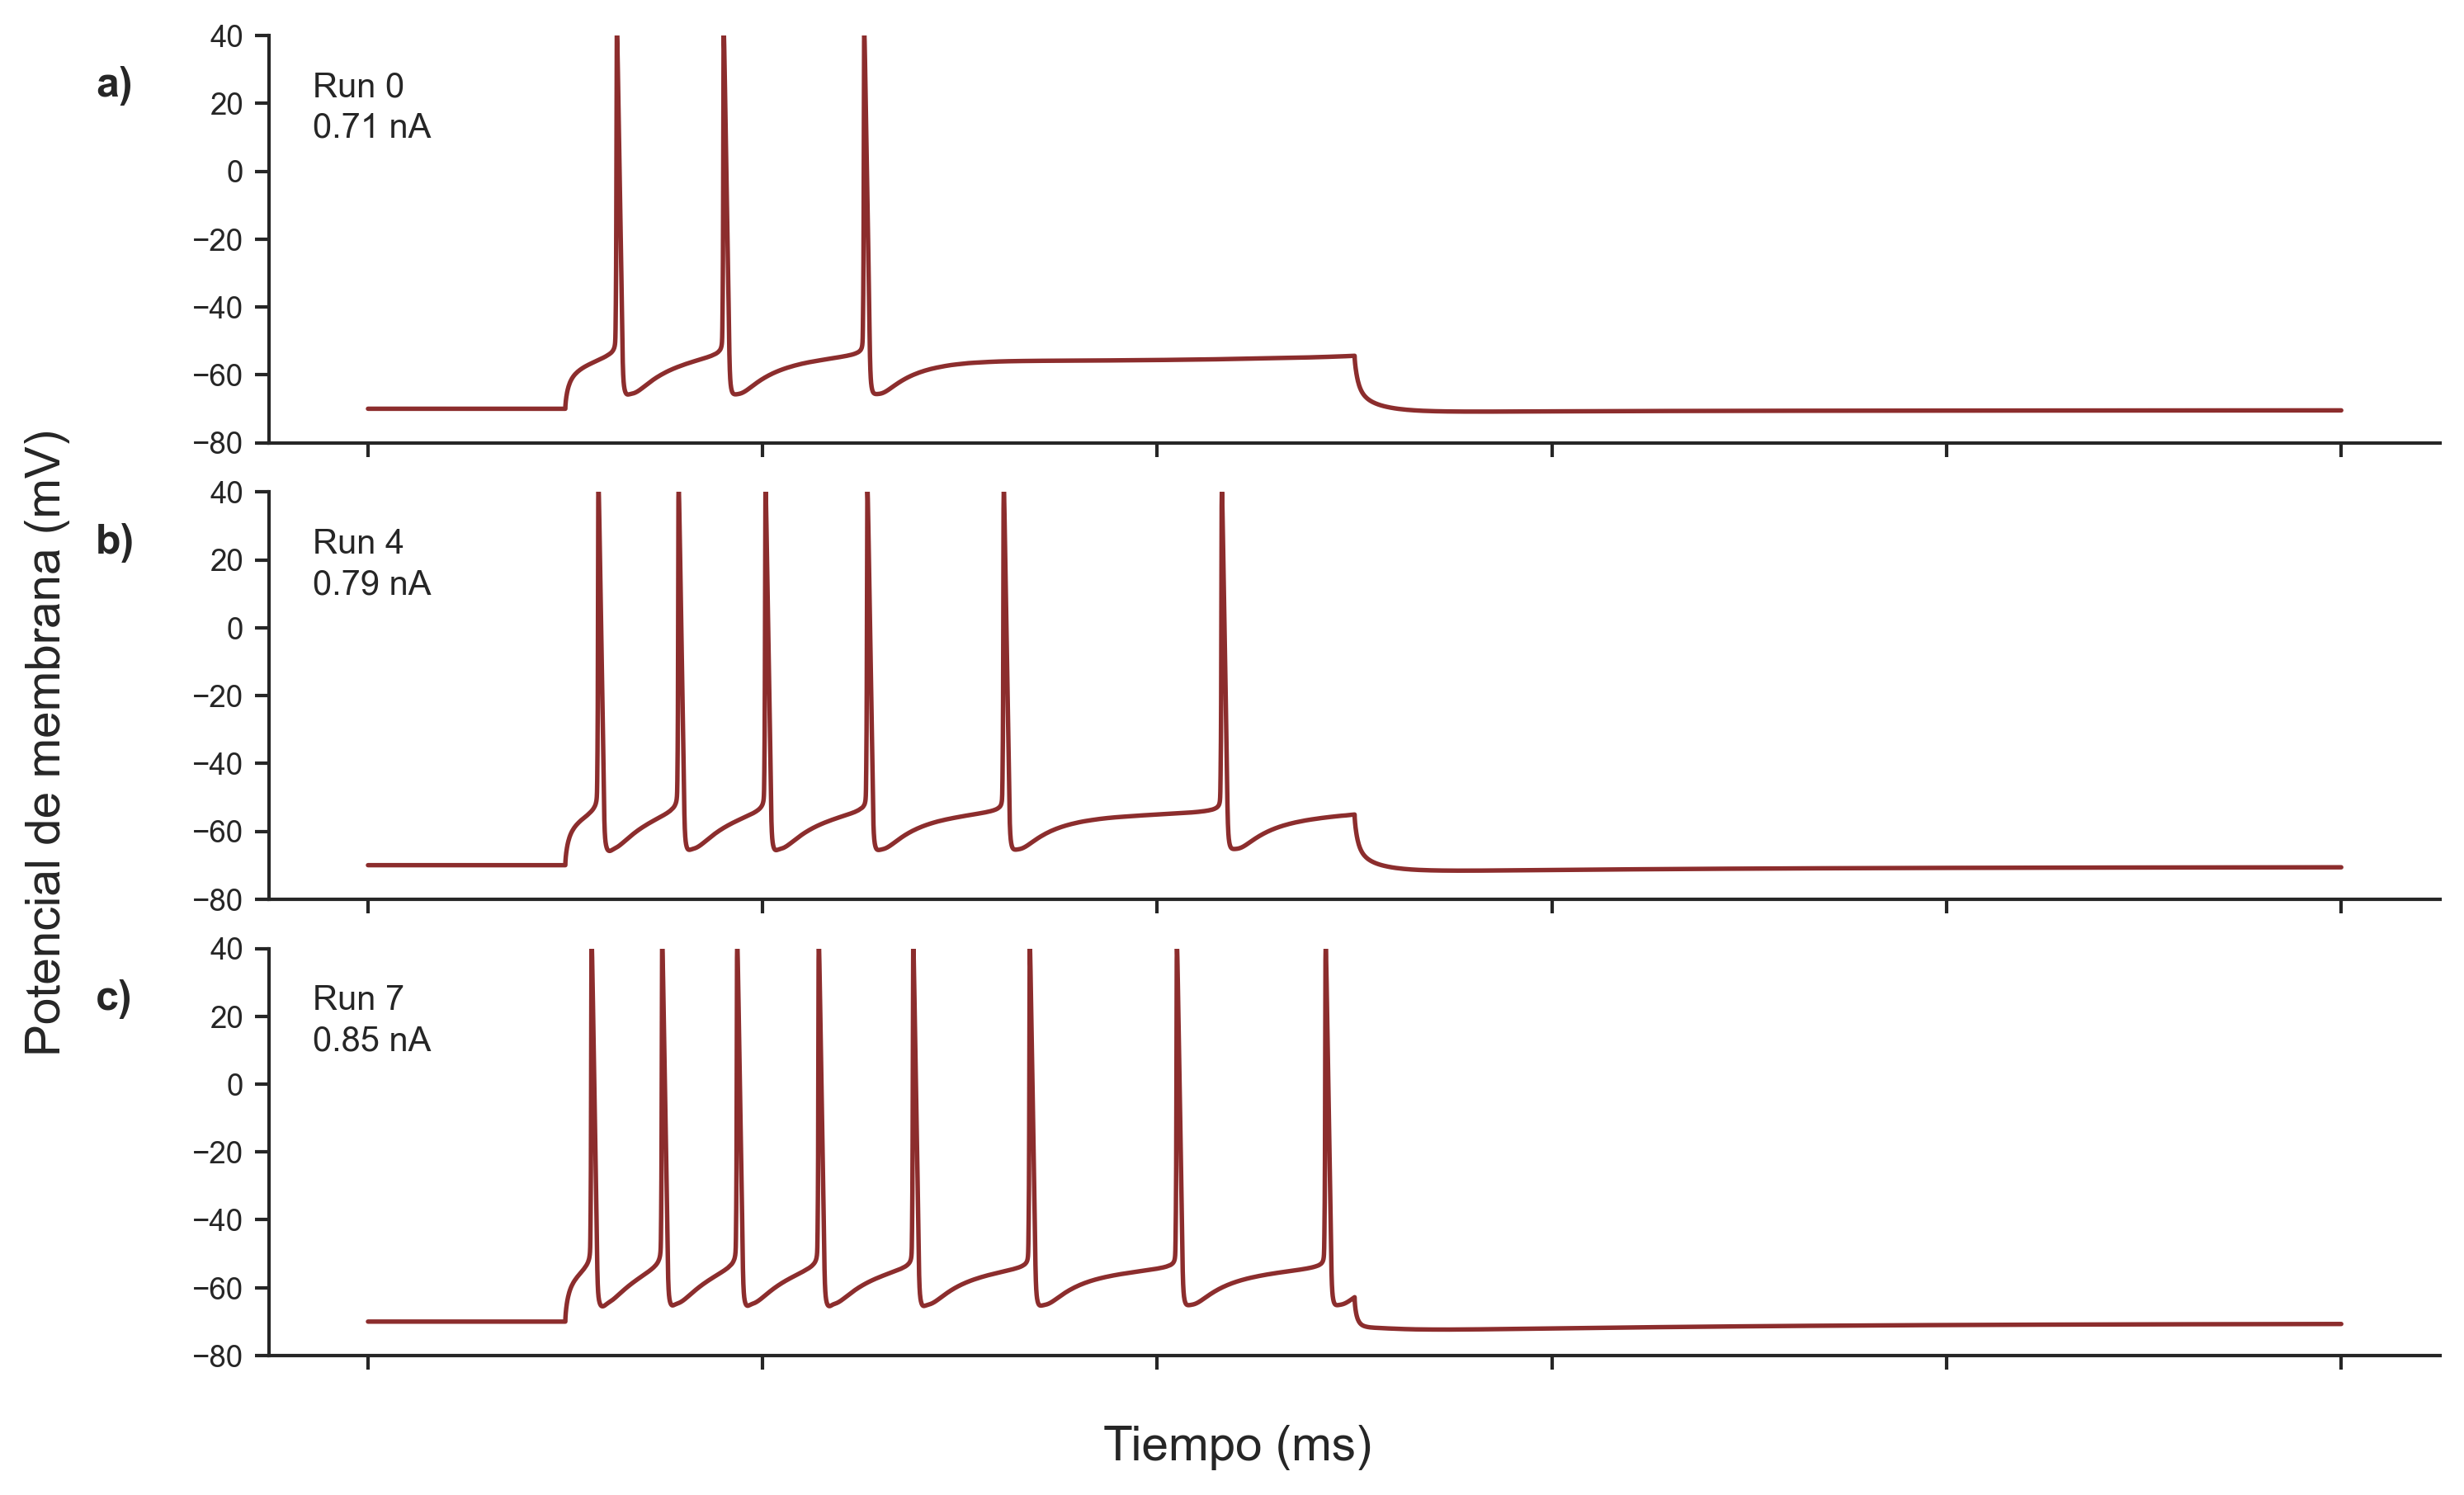
\includegraphics[width=0.65\textwidth]{../figs/selected_runs.png}
    \caption{Patrón de actividad neuronal obtenido en tres ejecuciones seleccionadas de la fase exploratoria, con distintos valores de corriente inyectada.}
    \label{fig:selectedruns}
\end{wrapfigure}

\textbf{Análisis de corrientes post-hiperpolarización.} De nuevo mediante un análisis visual, se analizó que el modelo inicial mostraba en la actividad de la neurona una hiperpolarización posterior al disparo correspondiente a las corriente media de post hiperpolarización, mAHP. Había cierto fenómeno de recuperación lenta tras la hiperpolarización, sAHP, como puede verse en la Figura \ref{fig:sAHP}, sin ser especialmente marcado.
Por este motivo, el modelo inicial se desarrolló para incluir un canal de potasio dependiente de calcio de modulación lenta (“canal de sAHP”), frente al ya existente de modulación rápida (tipo BK). Se implementó con dinámica lenta y activación sigmoidal dependiente de calcio intracelular. El modelo incorporó constantes temporales diferenciadas de activación y desactivación para reproducir la hiperpolarización lenta observada tras actividad neuronal repetida; el detalle de la definición se incluye en el Anexo 2. La diferencia en el patrón de recuperación tras la inclusión de este canal se muestra en la Figura \ref{fig:sAHP}.

\begin{figure}[h]
    \centering
    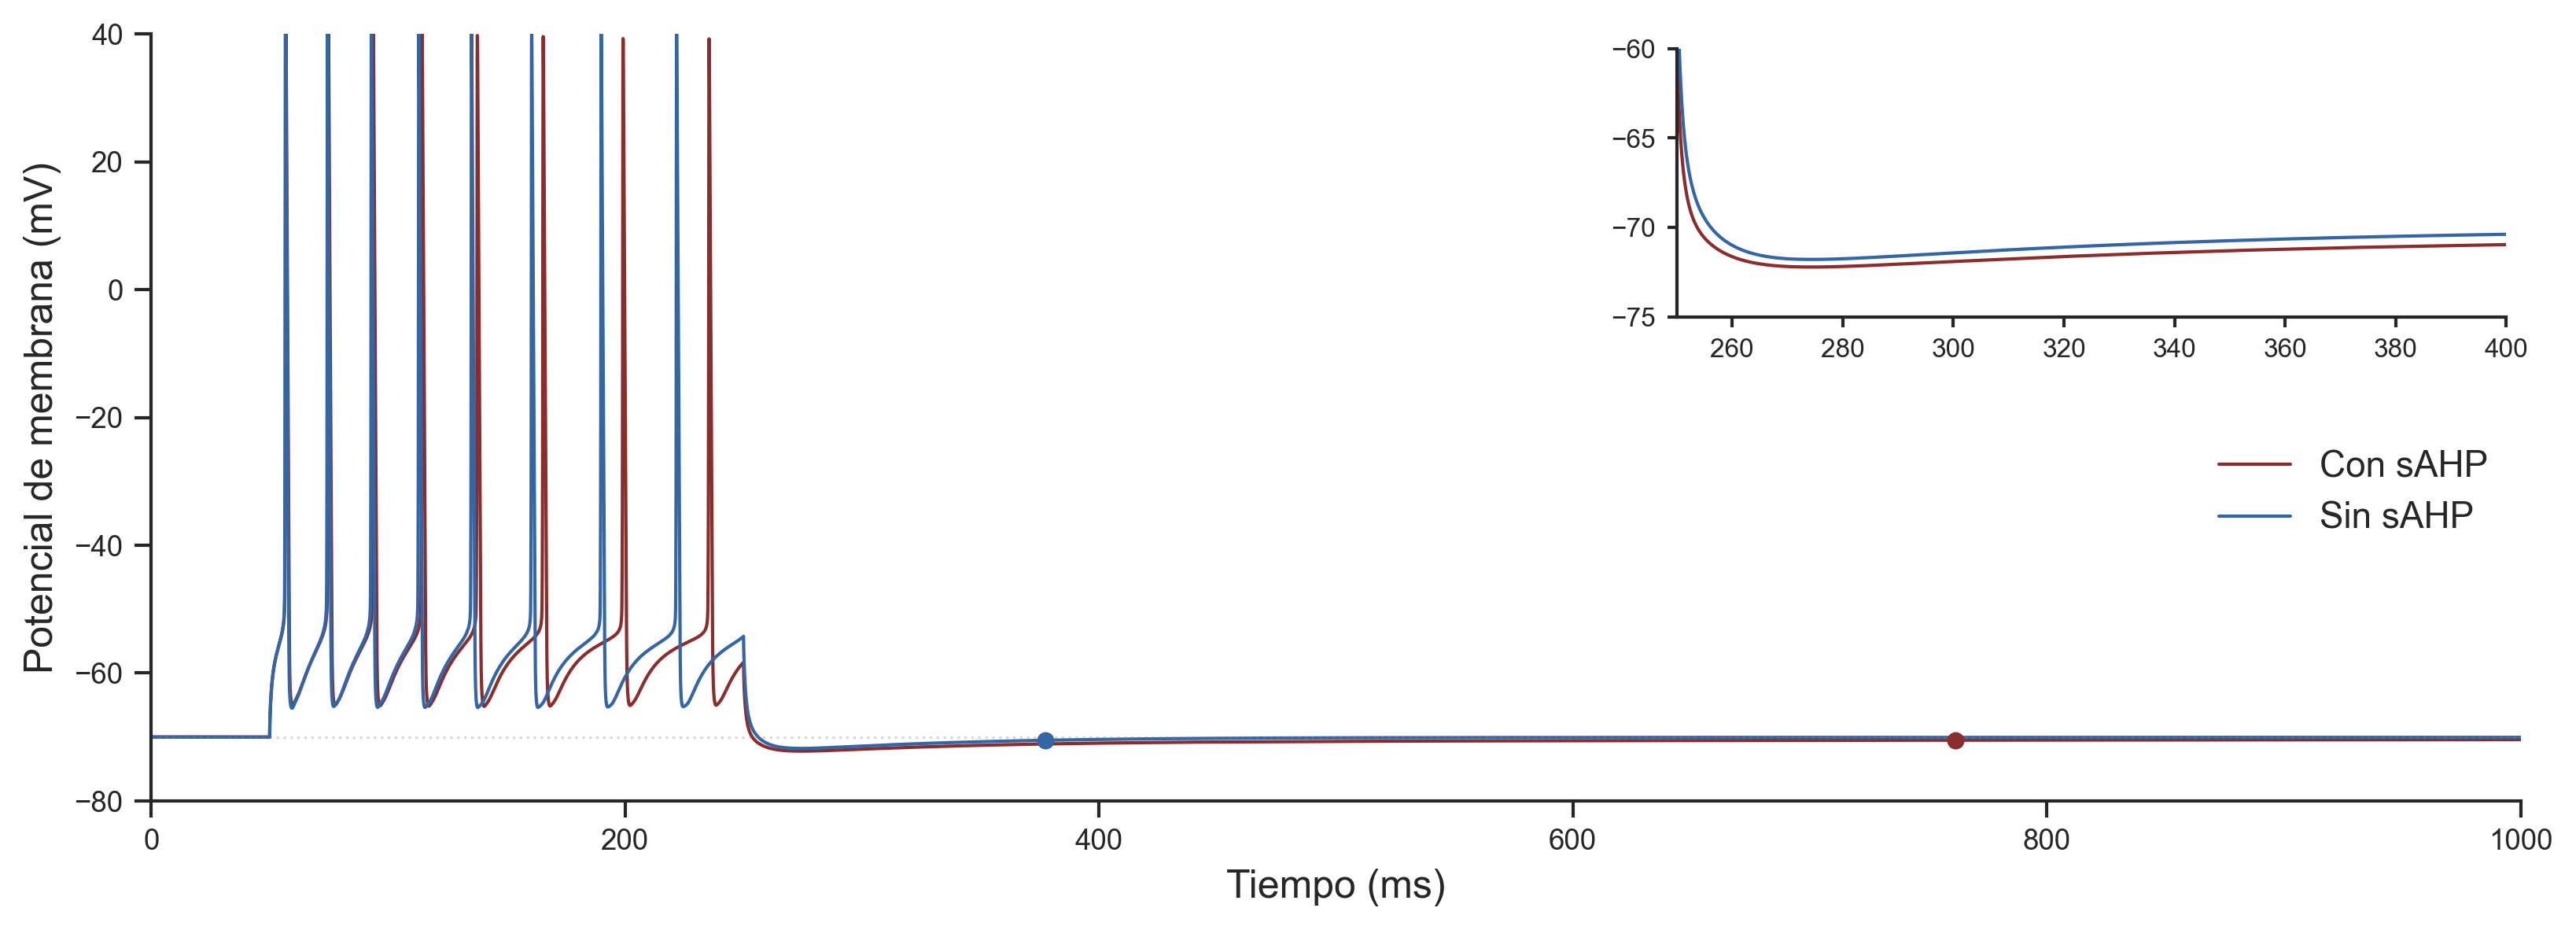
\includegraphics[width=0.85\textwidth]{../figs/run_comparison.png}
    \caption{Patrón de actividad neuronal antes y después de la inclusión del canal de sAHP, mostrando una hiperpolarización más prolongada tras la fase de disparo. Se marcan con un círculo los momentos temporales en los que el voltaje de membrana vuelve a un valor de -70.5 mV. Como se menciona en el texto, la recuperación es más larga tras la inclusión del mecanismo de sAHP.}
    \label{fig:sAHP}
\end{figure}

\textbf{\textit{Bursts} periódicos.} Debido al objetivo de realizar un análisis de la frecuencia de la actividad oscilatoria, era necesario poder simular no sólo un evento de disparos rápidos, sino varios consecutivos, y observar el patrón de recuperación \textit{inter-burst}. A este efecto, y contando con las limitaciones de la estimulación descrita (corriente inyectada directamente en la neurona), se creó un estímulo condicionado: una vez el voltaje de membrana volvía a un valor cercano al reposo, definido como (\textit{Vreposo} - 0,1) mV inicialmente, se disparaba un nuevo estímulo de corriente. Este patrón de estimulación simulaba el fenómeno fisiológico del periodo refractario, en el que la neurona no puede volver a disparar hasta recuperarse de la hiperpolarización, y se refleja en la Figura \ref{fig:freq_comparison}. 
Además, se analizó la frecuencia de esta actividad rítmica. Para ello, se obtuvo la media de la ventana temporal entre los periodos de \textit{bursting}. A partir de este valor, al calcular su inverso se obtuvo un valor de la frecuencia.

\begin{figure}[h]
    \centering
    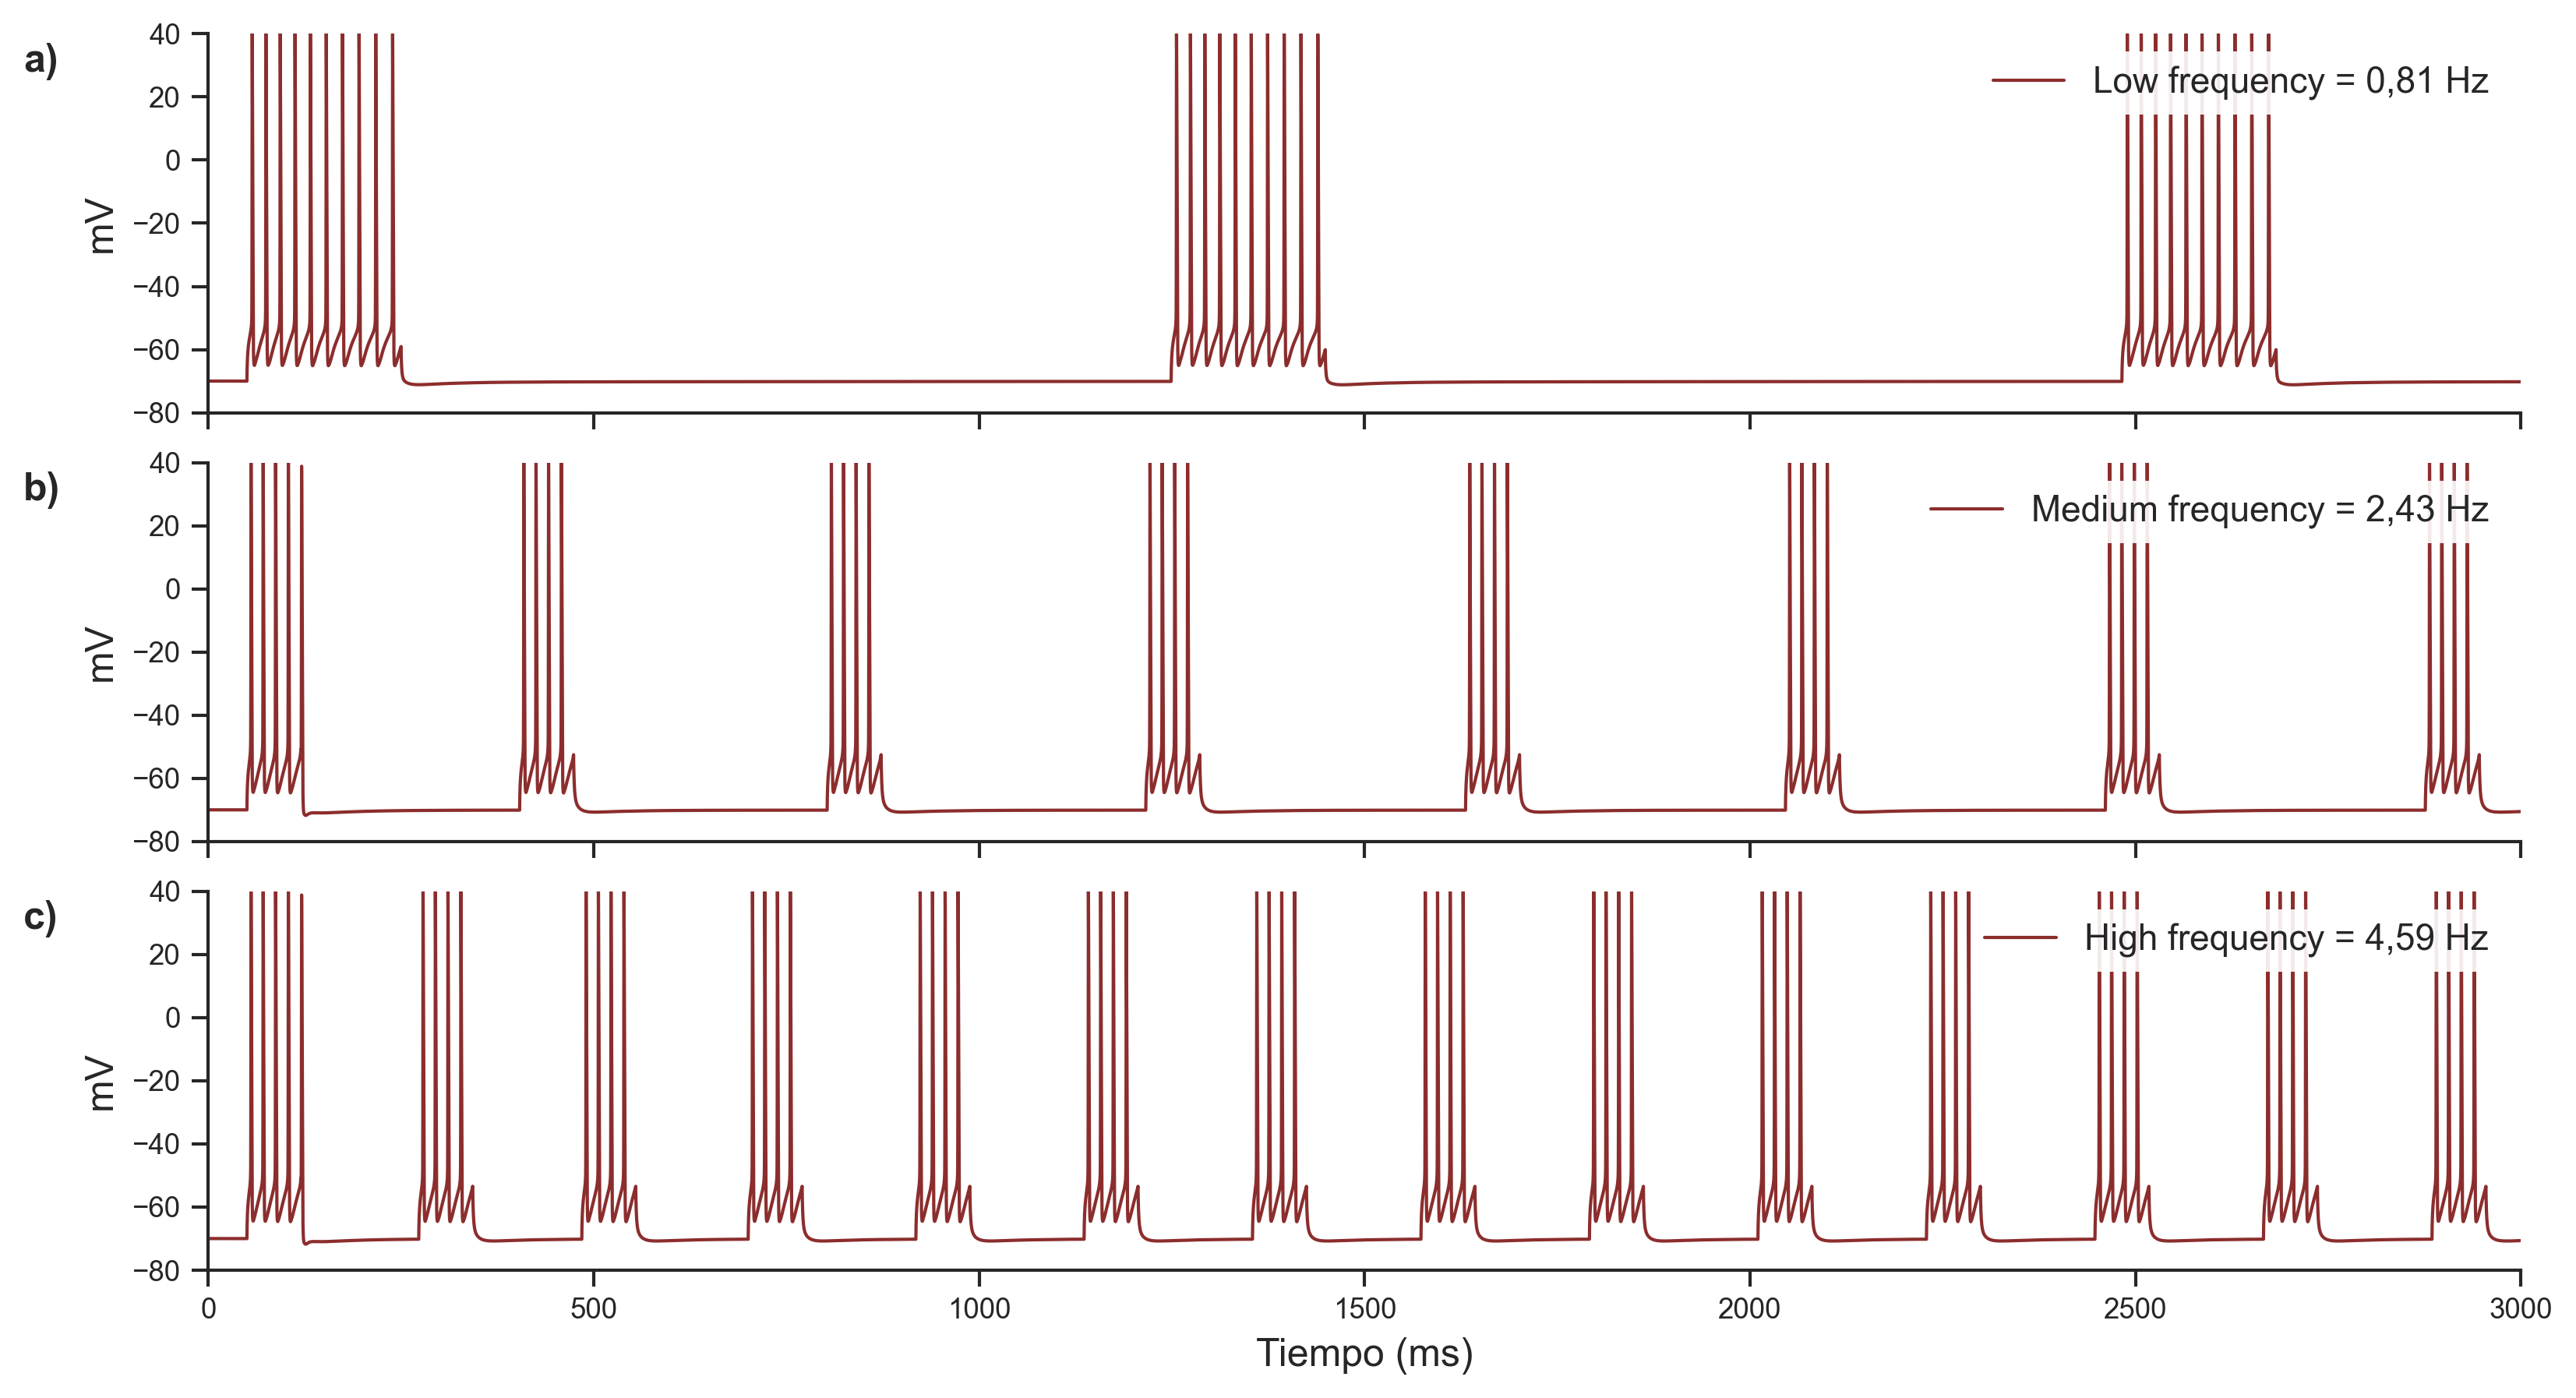
\includegraphics[width=0.85\textwidth]{../figs/freq_comparison.png}
    \caption{Patrón de actividad neuronal con estímulo condicionado al retorno al reposo, mostrando la aparición de \textit{bursts} periódicos. La frecuencia obtenida inicialmente fue de 0,81 Hz (a), y tras la modificación de parámetros para aumentar la frecuencia, se obtuvo una frecuencia de 4,59 Hz (c).}
    \label{fig:freq_comparison}
\end{figure}

\textbf{Adaptación de la frecuencia.} Como se refleja en la Figura \ref{fig:freq_comparison}, la frecuencia obtenida inicialmente fue de 0,81 Hz (a). La actividad relevante para el estudio se encuentra en la banda theta de frecuencias (4 - 8 Hz), por lo que se modificaron los parámetros de nuevo con el objetivo de aumentarla. Para ello, se modificaron parámetros de estimulación como la duración y amplitud, y la condición de vuelta al reposo, así como el parámetro de la sAHP, llegando a obtener una frecuencia de 4,59 Hz (c) que se sitúa en la banda de interés.

\textbf{Componente astrocitario.} La cadena de acción del astrocito se condensó en un último paso funcional en el que el astrocito de manera simplificada actúa aumentando el calcio intracelular. Se incorporó un evento de estimulación en el modelo que reflejase esta acción, a través de la modificación del parámetro gcal - un parámetro que refleja la capacidad de entrada de calcio a través de canales de calcio dependientes de voltaje tipo L, y que simplificadamente simula una mayor eficacia de entrada de calcio neuronal. El patrón de estimulación inicialmente se definió como una actividad sinusoidal de ventanas temporales largas (s) en comparación con la de la neurona (ms). Sin embargo, la componente negativa de la sinusoidal representa una falsa inhibición fisiológica del astrocito hacia la neurona, por lo que se modificó para solo simular la componente positiva, intercalada con momentos de pausa de actividad astrocitaria (ver Anexo 3, y Figura \ref{fig:astro_comparison}). La amplitud de la señal sinusoidal determinaba la magnitud de la modulación astrocitaria sobre gcal, mientras que el período controlaba la escala temporal de las oscilaciones gliales simuladas. Ambos parámetros fueron simulados con distintos valores, los resultados se presentan en el Anexo 4.

\begin{figure}[h]
    \centering
    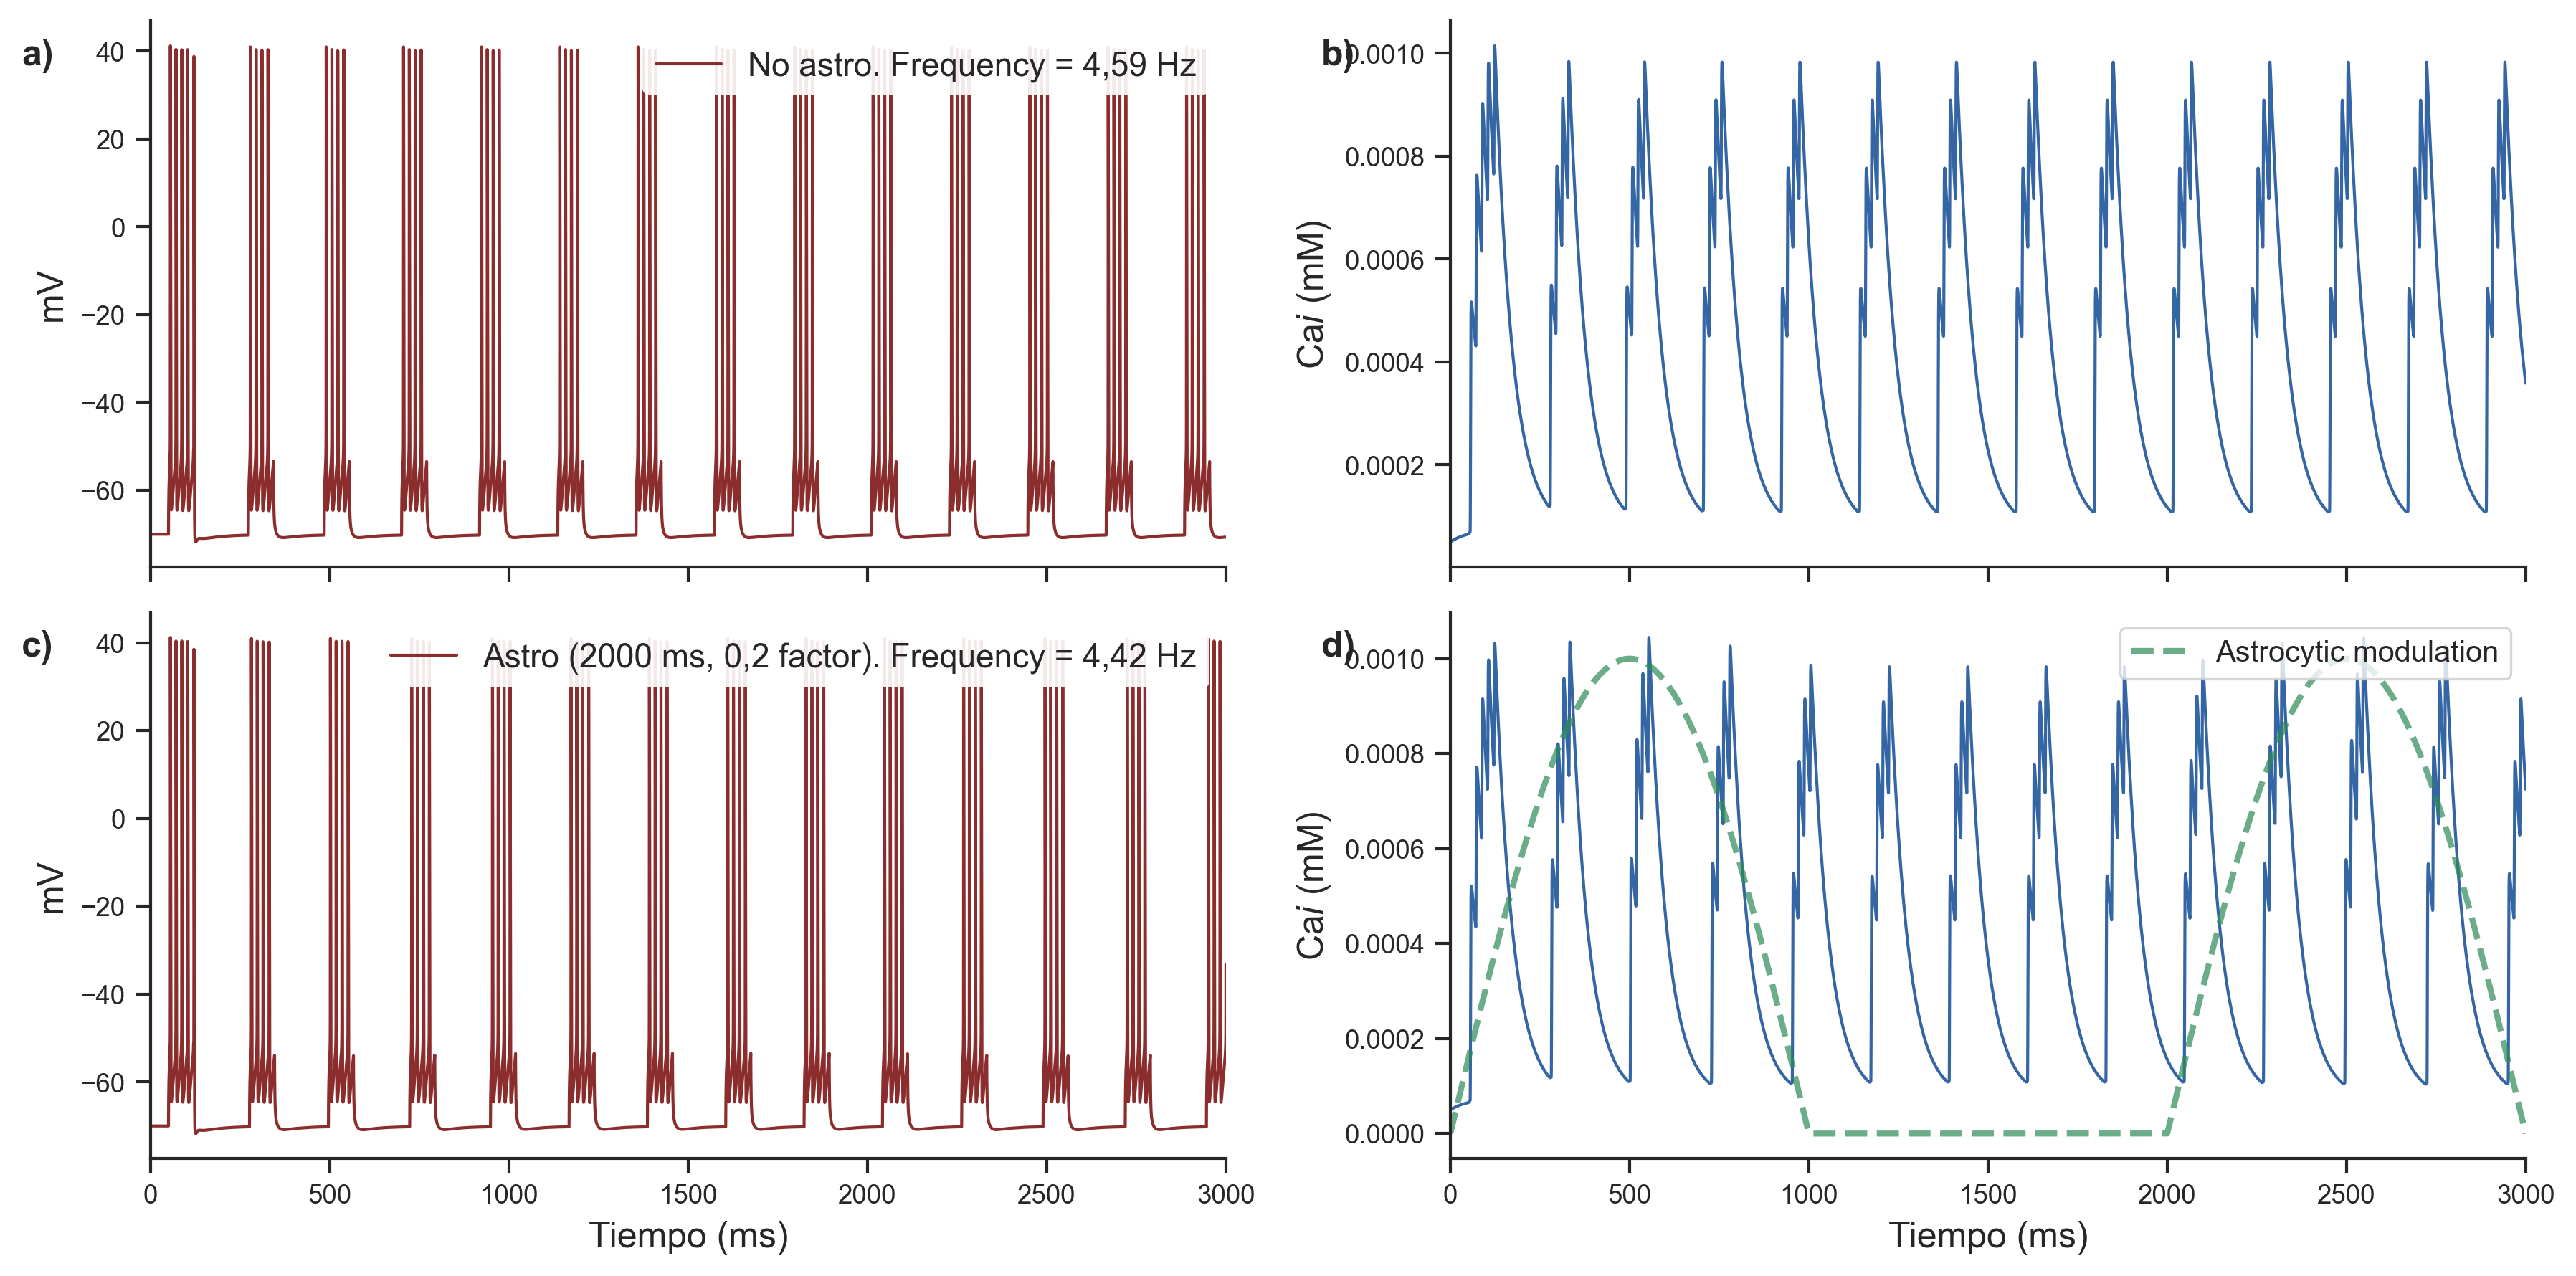
\includegraphics[width=0.85\textwidth]{../figs/astro_comparison.png}
    \caption{Patrón de actividad neuronal junto con niveles de calcio intracelular (cai), con y sin modulación astrocitaria, mostrando cómo la modulación astrocitaria produce un descenso en la frecuencia de oscilación. Se incluye en verde la señal de modulación astrocitaria, que se superpone a la actividad neuronal.}
    \label{fig:astro_comparison}
\end{figure}

\subsection{Fase experimental}
Una vez obtenido un modelo capaz de simular eventos neuronales relevantes de \textit{bursting} en la banda de frecuencia theta, se pasó a la comparar la frecuencia oscilatoria en distintas condiciones experimentales. Los resultados se presentan en la Figura \ref{fig:astro_comparison_final}. La actividad astrocitaria de intensidad baja disminuye la frecuencia de oscilación, y a mayor intensidad, mayor el descenso.

\begin{figure}[h]
    \centering
    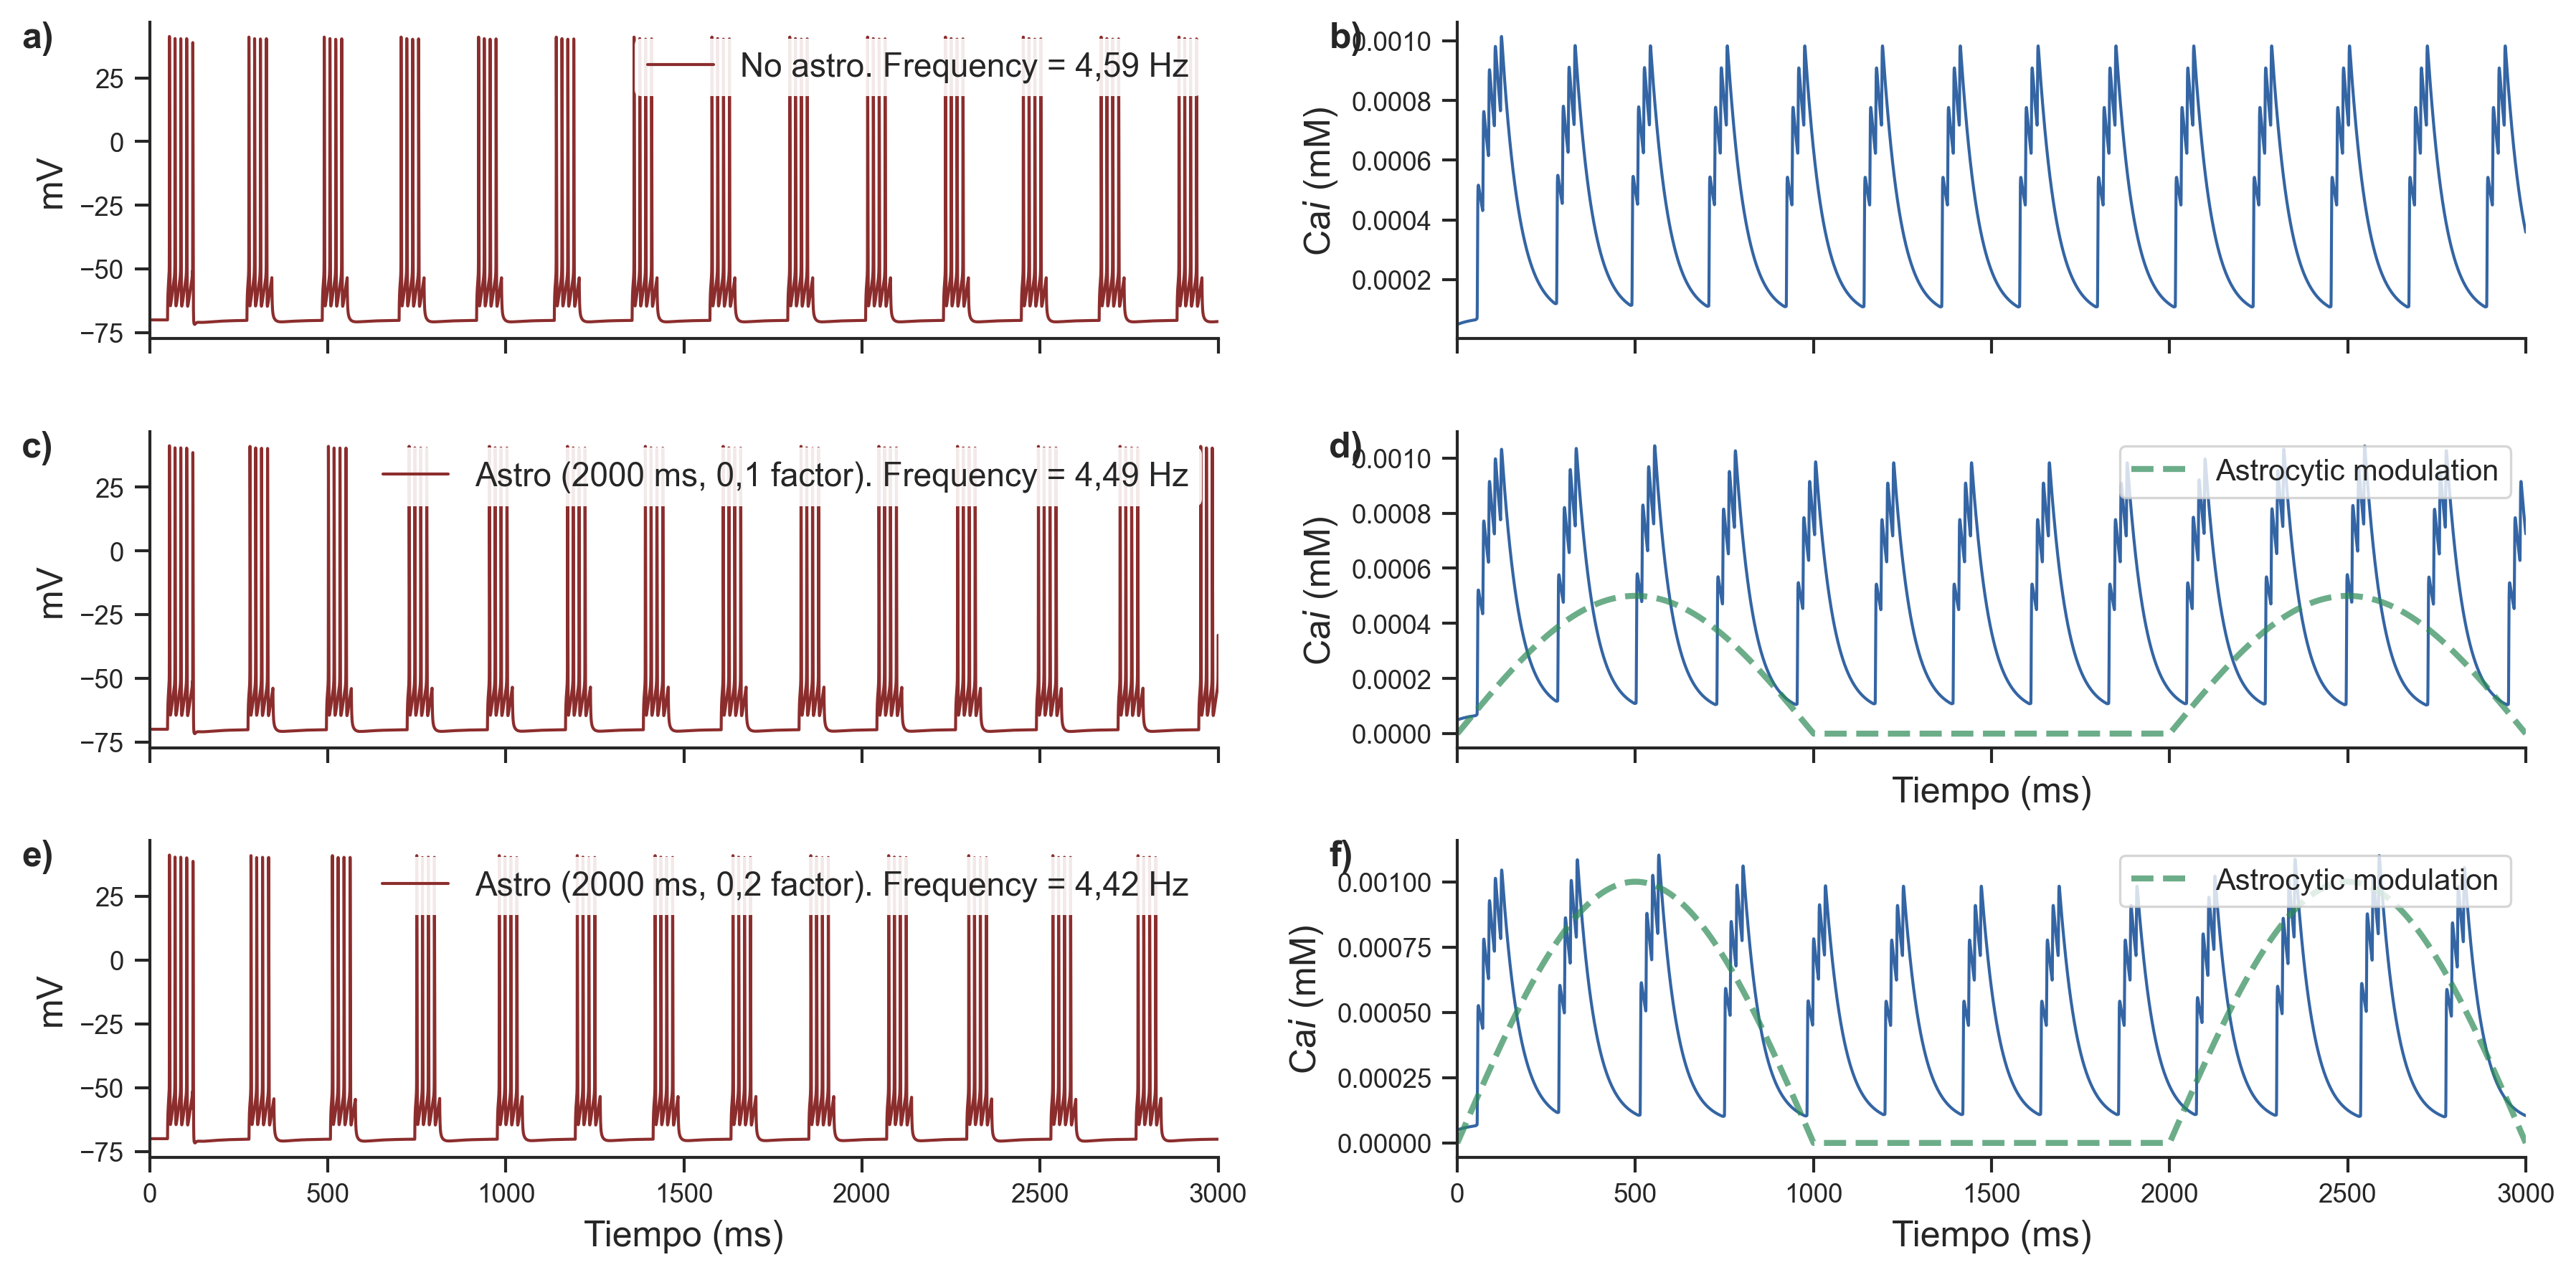
\includegraphics[width=0.95\textwidth]{../figs/astro_comparison_final.png}
    \caption{Patrón de actividad neuronal junto con niveles de calcio intracelular (cai) bajo distintas intensidades de modulación astrocitaria, mostrando cómo la modulación astrocitaria produce un descenso en la frecuencia de oscilación. Se incluye en verde la señal de modulación astrocitaria, que se superpone a la actividad neuronal. Como se menciona en el texto, a mayor intensidad de modulación astrocitaria, mayor el descenso en la frecuencia de oscilación.}
    \label{fig:astro_comparison_final}
\end{figure}

\section{Discusión}
En este trabajo se desarrolló un modelo computacional multicompartmental de una neurona piramidal CA1 orientado al estudio de las corrientes de post-hiperpolarización y de su influencia sobre la excitabilidad neuronal. Los resultados obtenidos sugieren que modulaciones lentas de la entrada de calcio, implementadas como una aproximación simplificada de la señalización astrocitaria, pueden alterar la dinámica temporal de la excitabilidad neuronal y modificar parcialmente los patrones oscilatorios de disparo. El modelo mostró que pequeñas variaciones en la entrada de calcio producen modificaciones sostenidas en la activación de corrientes lentas de potasio dependientes de calcio (sAHP). Debido a que estas corrientes contribuyen a la hiperpolarización prolongada tras trenes de potenciales de acción, cambios relativamente pequeños en la dinámica del calcio intracelular pueden traducirse en variaciones apreciables aunque pequeñas, en la frecuencia de disparo y en los intervalos entre \textit{bursts}. Estos resultados son consistentes con estudios previos que han relacionado la sAHP con mecanismos de adaptación neuronal y control de excitabilidad en neuronas CA1 hipocampales, donde la acumulación intracelular de calcio regula la duración de los periodos refractarios funcionales y la frecuencia de disparo sostenido (Madison et al., 1984; Sah et al., 2002; Golomb et al., 2006).

Las modulaciones periódicas introducidas en el modelo generaron cambios lentos en la excitabilidad basal de la neurona, produciendo ligeras variaciones en la distribución temporal de la actividad de disparo. Este efecto podría interpretarse como una forma de desplazamiento espectral (“\textit{spectral shift}”) de la actividad neuronal, en el sentido de una reorganización lenta de la frecuencia dominante de disparo alrededor de un estado basal. Esta interpretación resulta compatible con trabajos recientes que proponen que mecanismos gliales lentos pueden modular dinámicas oscilatorias neuronales sin necesidad de actuar directamente como generadores primarios del ritmo, sino alterando las propiedades intrínsecas que determinan la frecuencia de oscilación neuronal (Expósito et al., 2025). En este contexto, la modulación de corrientes dependientes de calcio podría constituir uno de los mecanismos celulares responsables de dichos desplazamientos dinámicos de frecuencia. 

Aunque el modelo implementa la actividad astrocitaria de manera simplificada mediante una modulación sinusoidal de la conductancia de canales de calcio, este enfoque pretende representar únicamente la escala temporal lenta característica de muchos procesos gliales. En condiciones fisiológicas, la señalización astrocitaria presenta dinámicas complejas, frecuentemente dependientes de calcio intracelular, liberación de gliotransmisores y regulación metabólica o iónica del entorno extracelular. Por tanto, el modelo no pretende reproducir de manera exacta la fisiología astrocitaria, sino explorar de forma controlada cómo modulaciones lentas de la excitabilidad podrían influir sobre mecanismos intrínsecos de adaptación neuronal.

El paradigma de estimulación empleado constituye una aproximación simplificada a la dinámica neuronal fisiológica. En las simulaciones, la estimulación era aplicada cuando la neurona retornaba aproximadamente al potencial de reposo, permitiendo estudiar de manera controlada la recuperación de la excitabilidad y la influencia de las corrientes IAHP sobre el disparo repetido. No obstante, en condiciones fisiológicas reales las neuronas reciben entradas sinápticas continuas y parcialmente superpuestas, de forma que la aparición de nuevos potenciales de acción depende del estado dinámico instantáneo de las corrientes iónicas, de la acumulación intracelular de calcio y del periodo refractario funcional de la membrana.

Otra limitación importante deriva de la propia escala del modelo. El presente trabajo se centró en una única neurona piramidal CA1 aislada, permitiendo analizar con detalle la interacción entre calcio intracelular, corrientes IAHP y excitabilidad intrínseca. Sin embargo, la actividad oscilatoria hipocampal emerge normalmente de la interacción coordinada entre múltiples poblaciones neuronales, incluyendo neuronas piramidales, interneuronas inhibitorias y astrocitos, organizadas en redes. Por tanto, el modelo no reproduce directamente fenómenos colectivos de sincronización neuronal ni dinámicas de red complejas. 

Futuros trabajos podrían extender el modelo hacia configuraciones multicelulares que incorporen interacciones sinápticas explícitas y mecanismos gliales más detallados, incluyendo procesos de gliotransmisión, regulación extracelular de potasio o señalización mediada por ATP y adenosina. La implementación de redes neuronales permitiría además estudiar cómo modificaciones intrínsecas de la excitabilidad, mediadas por corrientes dependientes de calcio, podrían traducirse en cambios coordinados de la actividad oscilatoria a nivel poblacional. Modelos previos han mostrado que simulaciones de cientos de neuronas permiten analizar fenómenos de sincronización mediante representaciones tipo \textit{raster plot} y estudiar la aparición de ritmos colectivos asociados a determinadas bandas de frecuencia (Sanjay et al., 2015). En consecuencia, los resultados presentados aquí deben considerarse principalmente como evidencia exploratoria acerca de posibles mecanismos celulares de modulación oscilatoria, más que como una reproducción cuantitativa completa de la fisiología hipocampal.


% ------------------------------------------------
% VALORACIÓN PERSONAL
% ------------------------------------------------
\chapter{Valoración personal}

Las prácticas realizadas han sido de investigación en un centro externo, el CSIC, y en concreto el Instituto Cajal. Han sido una oportunidad muy valiosa de entrar en contacto con áreas de la neuropsicología que han sido solo estudiadas a alto nivel durante la carrera. 

Las actividades realizadas han sido formativas, empezando desde una aproximación más general al tema, hasta llegar al detalle de lo que se requería estudiar. Se ha podido hacer un aprendizaje progresivo que ha permitido la adquisición de conocimientos más complejos que no hubiesen sido adquiridos con la misma facilidad fuera de este entorno. El propósito de resolver un problema como es el de desarrollar un modelo computacional que conceptualmente sea una aproximación lo más fisiológicamente realista ha sido muy útil para poder aplicar los conocimientos que se iban adquiriendo a lo largo del tiempo. 

El trabajo ha sido complejo al partir de una base más psicológica que neurocientífica, pero el resultado final lo valoro como satisfactorio tanto en un plano técnico, ya que se ha conseguido avanzar en el propósito inicial y se han obtenido unos resultados interesantes, como en el plano personal, al haber podido trabajar en un área fuera del área de comfort académica. 

Finalmente, las prácticas han sido un trabajo duro debido al solape en el tiempo con responsabilidades del último curso como el TFG y otras responsabilidades laborales. A pesar de ello, he disfrutado realizándolas y han estimulado mi curiosidad científica, motivándome para proseguir en esta área de investigación.


% ------------------------------------------------
% BIBLIOGRAFÍA
% ------------------------------------------------
\chapter{Bibliografía}
Araque, A., Parpura, V., Sanzgiri, R. P., \& Haydon, P. G. (1999). Tripartite synapses: Glia, the unacknowledged partner. \textit{Trends in Neurosciences, 22}(5), 208--215. \url{https://doi.org/10.1016/S0166-2236(98)01349-6}

Bean, B. (2007). The action potential in mammalian central neurons. \textit{Nature Reviews Neuroscience, 8}, 451--465. \url{https://doi.org/10.1038/nrn2148}

Bellot-Saez, A., Kékesi, O., Morley, J. W., \& Buskila, Y. (2017). Astrocytic modulation of neuronal excitability through K+ spatial buffering. \textit{Neuroscience \& Biobehavioral Reviews, 77}, 87--97. \url{https://doi.org/10.1016/j.neubiorev.2017.03.002}

Chen, S., Yue, C., \& Yaari, Y. (2005). A transitional period of Ca2+-dependent spike afterdepolarization and bursting in developing rat CA1 pyramidal cells. \textit{The Journal of Physiology, 567}(Pt 1), 79--93. \url{https://doi.org/10.1113/jphysiol.2005.084590}

Expósito, S., Alberquilla, S., \& Martín, E. D. (2025). Astrocyte-interneuron interplay tunes neuronal excitability by enhancing the slow Ca2+-activated K+ current. \textit{Progress in Neurobiology, 251}, 102806. \url{https://doi.org/10.1016/j.pneurobio.2025.102806}

Faber, E. S., \& Sah, P. (2003). Calcium-activated potassium channels: Multiple contributions to neuronal function. \textit{The Neuroscientist, 9}(3), 181--194. \url{https://doi.org/10.1177/1073858403009003011}

Golomb, D., Yue, C., \& Yaari, Y. (2006). Contribution of persistent Na+ current and M-type K+ current to somatic bursting in CA1 pyramidal cells: Combined experimental and modeling study. \textit{Journal of Neurophysiology, 96}(4), 1912--1926. \url{https://doi.org/10.1152/jn.00205.2006}

Haydon, P. G. (2001). Glia: Listening and talking to the synapse. \textit{Nature Reviews Neuroscience, 2}, 185--193. \url{https://doi.org/10.1038/35058528}

Lancaster, B., \& Adams, P. R. (1986). Calcium-dependent current generating the afterhyperpolarization of hippocampal neurons. \textit{Journal of Neurophysiology, 55}(6), 1268--1282. \url{https://doi.org/10.1152/jn.1986.55.6.1268}

Leung, L. W., \& Yim, C. Y. (1991). Intrinsic membrane potential oscillations in hippocampal neurons in vitro. \textit{Brain Research, 553}(2), 261--274. \url{https://doi.org/10.1016/0006-8993(91)90834-I}

Madison, D. V., \& Nicoll, R. A. (1984). Control of the repetitive discharge of rat CA1 pyramidal neurones in vitro. \textit{The Journal of Physiology, 354}, 319--331. \url{https://doi.org/10.1113/jphysiol.1984.sp015378}

Manara, E., Mele, A., \& Migliore, M. (2025). In silico investigation of the puzzling dopamine effects on excitability and synaptic plasticity in hippocampal CA1 pyramidal neurons. \textit{Scientific Reports, 15}, 32822. \url{https://doi.org/10.1038/s41598-025-17694-8}

Pedarzani, P., \& Stocker, M. (2008). Molecular and cellular basis of small- and intermediate-conductance, calcium-activated potassium channel function in the brain. \textit{Cellular and Molecular Life Sciences, 65}, 3196--3217. \url{https://doi.org/10.1007/s00018-008-8216-x}

Perea, G., \& Araque, A. (2007). Astrocytes potentiate transmitter release at single hippocampal synapses. \textit{Science, 317}(5841), 1083--1086. \url{https://doi.org/10.1126/science.1144640}

Perea, G., Navarrete, M., \& Araque, A. (2009). Tripartite synapses: Astrocytes process and control synaptic information. \textit{Trends in Neurosciences, 32}(8), 421--431. \url{https://doi.org/10.1016/j.tins.2009.05.001}

Poskanzer, K. E., \& Yuste, R. (2016). Astrocytes regulate cortical state switching in vivo. \textit{Proceedings of the National Academy of Sciences, 113}(19), E2675--E2684. \url{https://doi.org/10.1073/pnas.1520759113}

Sah, P., \& Faber, E. S. (2002). Channels underlying neuronal calcium-activated potassium currents. \textit{Progress in Neurobiology, 66}(5), 345--353. \url{https://doi.org/10.1016/S0301-0082(02)00004-7}

Sanjay, M., Neymotin, S. A., \& Krothapalli, S. B. (2015). Impaired dendritic inhibition leads to epileptic activity in a computer model of CA3. \textit{Hippocampus, 25}, 1336--1350.

Semyanov, A., Henneberger, C., \& Agarwal, A. (2020). Making sense of astrocytic calcium signals: From acquisition to interpretation. \textit{Nature Reviews Neuroscience, 21}, 551--564. \url{https://doi.org/10.1038/s41583-020-0361-8}

Tzingounis, A. V., \& Nicoll, R. A. (2008). Contribution of KCNQ2 and KCNQ3 to the medium and slow afterhyperpolarization currents. \textit{Proceedings of the National Academy of Sciences, 105}, 19974--19979. \url{https://doi.org/10.1073/pnas.0810535105}

Volterra, A., \& Meldolesi, J. (2005). Astrocytes, from brain glue to communication elements: The revolution continues. \textit{Nature Reviews Neuroscience, 6}, 626--640. \url{https://doi.org/10.1038/nrn1722}


% ------------------------------------------------
% ANEXOS
% ------------------------------------------------
\chapter{Anexos}

\section{Anexo 1. Gráficas de exploración de valor de estimulación.}
\vspace{-0.5em}
\begin{center}
    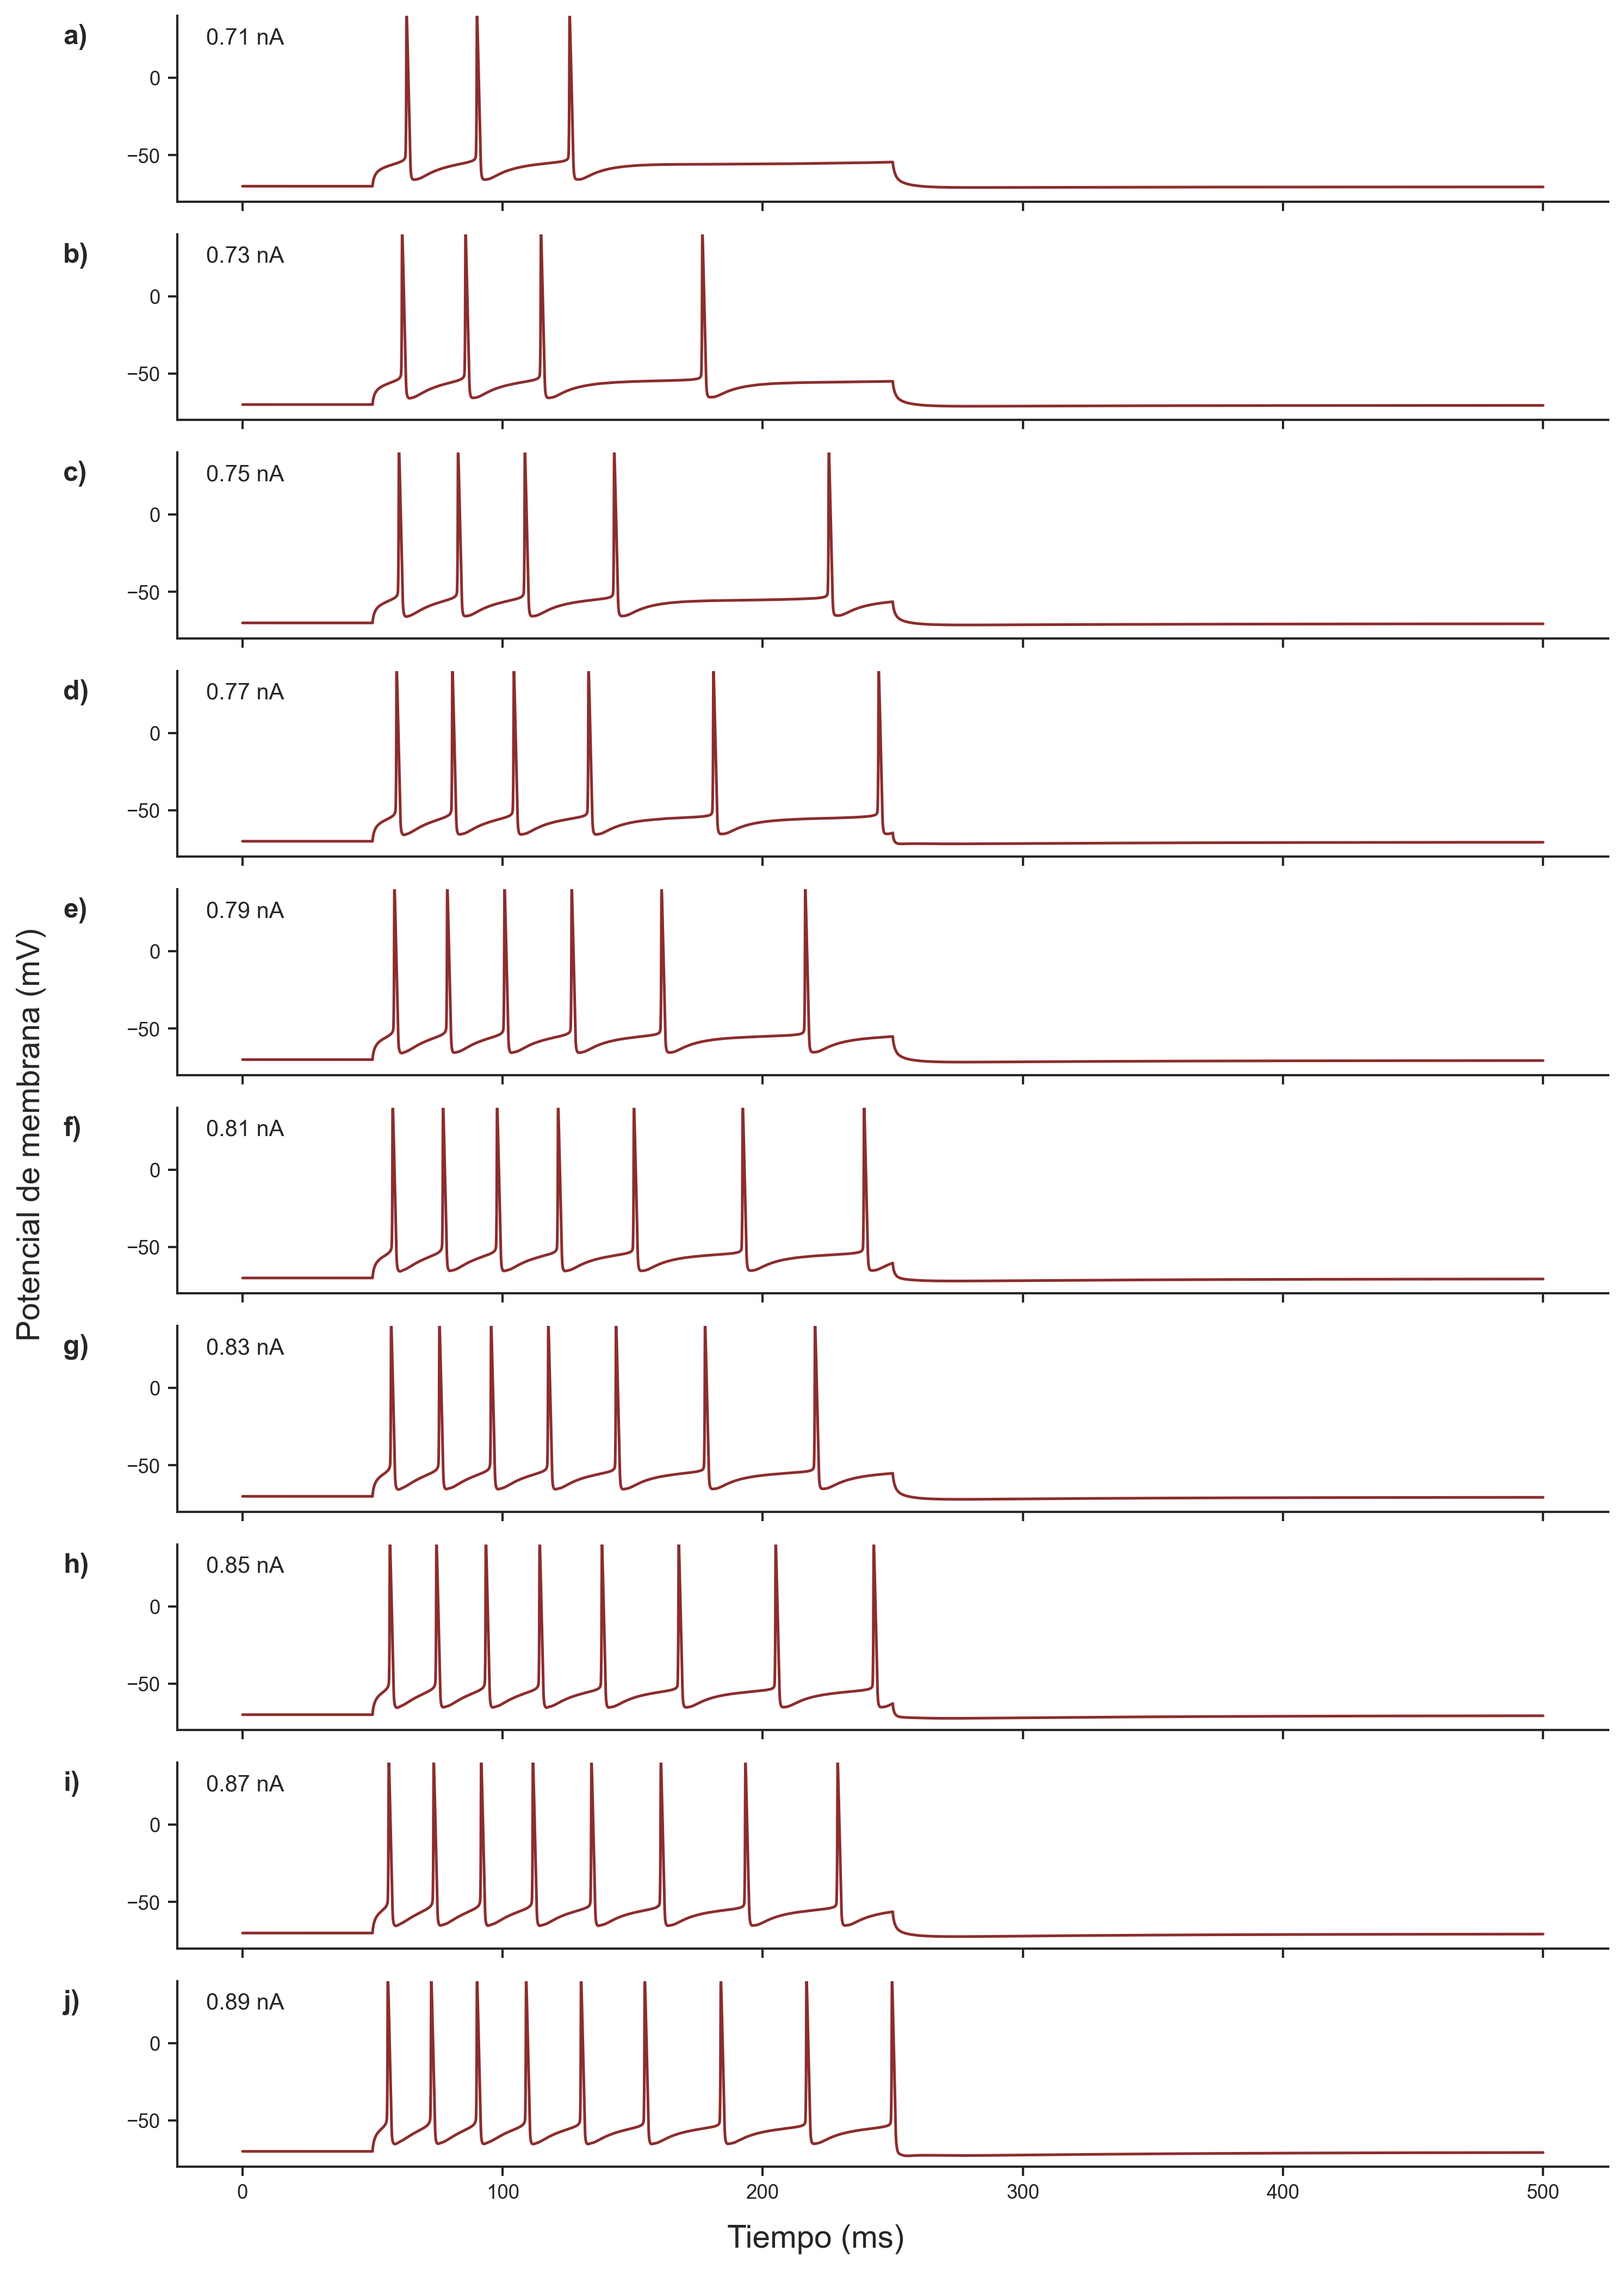
\includegraphics[width=0.82\textwidth]{../figs/all_runs.png}
\end{center}

\textbf{Figura A1.} Gráficas de actividad neuronal en diferentes condiciones de estimulación, mostradas en cada gráfica.Parámetros usados: Vrest = -70 mV, dt = 0.1, stim IClamp en ventana de 50 ms a 250 ms, tstop = 500 ms. Canales incluidos y sus parámetros: gna = 0.043, gkdr = 0.025, ghd = 0.0000011, gkm = 0.00002, gcat = 0.00004, gahp = 0.001, gcak = 0.000021, gcal = 0.002 (sin componente de sAHP).

\section{Anexo 2. Definición de canal de potasio activado por calcio (canal de sAHP).}

\begin{lstlisting}[caption=Código .hoc para el canal sAHP.]
TITLE slow K-AHP channel (no Ca filter, monotonic decay)
NEURON {
    SUFFIX KsAHP
    USEION k READ ek WRITE ik
    USEION ca READ cai
    RANGE gbar, ik, gksahp
}
UNITS {
    (mA) = (milliamp)
    (mV) = (millivolt)
}
PARAMETER {
    gbar = 0.001 (mho/cm2)
    tau_rise = 100 (ms)    : subida relativamente rapida
    tau_decay = 800 (ms)   : bajada lenta (sAHP real)
    n = 4
    kD = 0.0004 (mM)
    cai0 = 50e-6 (mM)
    ek (mV)
}
STATE {
    w   : activacion del canal
}
ASSIGNED {
    ik (mA/cm2)
    gksahp (mho/cm2)
    cai (mM)
    winf
    ca_eff
}
BREAKPOINT {
    SOLVE states METHOD cnexp
    gksahp = gbar * w
    ik = gksahp * (v - ek)
}
INITIAL {
    w = 0
}
DERIVATIVE states {
    : Ca efectivo (solo por encima del basal)
    ca_eff = cai - cai0
    if (ca_eff < 0) {
        ca_eff = 0
    }
    : activacion tipo Hill
    winf = ca_eff^n / (ca_eff^n + kD^n)
    : cinetica asimetrica
    if (winf > w) {
        w' = (winf - w)/tau_rise
    } else {
        w' = (winf - w)/tau_decay
    }
}

\end{lstlisting}

El canal KsAHP fue implementado como una corriente de potasio dependiente de calcio intracelular orientada a reproducir la componente lenta de la afterhyperpolarization (sAHP). La conductancia máxima del canal (gbar) determina la intensidad máxima de la corriente hiperpolarizante generada.

La activación del canal depende de la concentración intracelular de calcio (cai) mediante una función de Hill, donde $k_D$ representa la concentración de calcio necesaria para alcanzar una activación semimáxima del canal, mientras que el parámetro $n$ controla el grado de cooperatividad de la activación dependiente de calcio. Valores elevados de $n$ producen una transición más abrupta entre estados cerrados y abiertos del canal.

El modelo considera únicamente incrementos de calcio por encima de un nivel basal (cai0), definido como la concentración intracelular de calcio en reposo. De este modo, la activación del canal depende específicamente de la acumulación de calcio asociada a la actividad neuronal repetida.

La variable dinámica w representa el grado de activación del canal y evoluciona temporalmente hacia un valor de equilibrio (winf) mediante constantes temporales diferenciadas para activación y desactivación. El parámetro tau\_rise controla la velocidad de apertura del canal ante aumentos de calcio intracelular, mientras que tau\_decay determina la velocidad de cierre tras la reducción del calcio. La utilización de una constante de desactivación más lenta reproduce la naturaleza prolongada de la sAHP observada experimentalmente.

La corriente resultante (ik) se calcula como una corriente de potasio dependiente tanto de la conductancia instantánea (gksahp) como de la diferencia entre el potencial de membrana y el potencial de equilibrio del potasio (ek).


\section{Anexo 3. Modelo matemático del componente astrocitario.}

\begin{lstlisting}[caption=Código .hoc para el canal sAHP.]
proc astro_cycle() { local astro_factor, current_gcal
    astro_wave = sin(2*3.14159*t/2000)
    if (astro_wave < 0) {
        astro_wave = 0
    }
    astro_factor = 1 + 0.1*astro_wave
    current_gcal = gcal * astro_factor
}
\end{lstlisting}

\newpage
\section{Anexo 4. Resultados de exploración de parámetros de estimulación y del astrocito, y las frecuencias asociadas.}
\begin{table}[h]
\centering
\small

\begin{tabular}{cccccc}
\toprule

Run &
\makecell{Frecuencia\\(Hz)} &
\makecell{Condición para\\estimulación (mV)} &
\makecell{Amplitud\\estímulo (nA)} &
\makecell{Duración\\estímulo (ms)} &
\makecell{$g_{ahp\_slow}$} \\

\midrule

1 & 0,81 & -70,1 & 0,85  & 200 & 0,00001 \\
2 & 2,43 & -70,1 & 0,935 & 70  & 0,000005 \\
3 & 4,59 & -70,2 & 0,935 & 70  & 0,000005 \\

\bottomrule
\end{tabular}

\caption{Resultados de frecuencia de \textit{burst} según distintos parámetros en la simulación de la estimulación sobre la neurona, y el valor de la sAHP.}
\label{tab:estimulos}

\end{table}

\begin{table}[h]
\centering
\small

\begin{tabular}{cccccc}
\toprule

Run &
\makecell{Frecuencia\\(Hz)} &
\makecell{Factor\\sinusoidal} &
\makecell{Periodo de\\sinusoidal (ms)} &
\makecell{Condición para\\estimulación (mV)} &
\makecell{$g_{ahp\_slow}$} \\

\midrule

1 & 4,49 & 0,1 & 2000 & -70,2 & 0,000005 \\
2 & 4,42 & 0,2 & 2000 & -70,2 & 0,000005 \\
3 & 4,52 & 0,1 & 1000 & -70,2 & 0,000005 \\
4 & 4,46 & 0,2 & 1000 & -70,2 & 0,000005 \\

\bottomrule
\end{tabular}

\caption{Resultados de frecuencia de \textit{burst} según distintos parámetros en la simulación de la estimulación astrocitaria sobre la neurona.}
\label{tab:astro_sim}

\end{table}



\end{document}